\documentclass[leqno, openany]{memoir}
\setulmarginsandblock{3.5cm}{3.5cm}{*}
\setlrmarginsandblock{3cm}{3.5cm}{*}
\checkandfixthelayout

% math
\usepackage{amsmath}
\usepackage{amssymb}
\usepackage{amsthm}
%\usepackage{MnSymbol}
\usepackage{bm}
\usepackage{accents}
\usepackage{mathtools}
\usepackage{tikz}
\usetikzlibrary{calc}
\usetikzlibrary{automata,positioning}
\usepackage{tikz-cd}
\usepackage{forest}
\usepackage{braket} 
\usepackage{listings}
\usepackage{mdframed}
\usepackage{verbatim}
\usepackage{physics} 
\usepackage{graphicx}
\graphicspath{{./}}

% font
\usepackage[sc]{mathpazo}
\usepackage{eulervm}
\usepackage[scaled=0.86]{berasans}
\usepackage{inconsolata}
\usepackage{microtype}

%CS packages
\usepackage{algorithmicx}
\usepackage{algpseudocode}
\usepackage{algorithm}

% typeset and bib
\usepackage[english]{babel} 
\usepackage[utf8]{inputenc} 
\usepackage[T1]{fontenc}
\usepackage[backend=biber, style=alphabetic]{biblatex}
\usepackage[bookmarks, colorlinks, breaklinks]{hyperref} 
\hypersetup{linkcolor=black,citecolor=black,filecolor=black,urlcolor=black}
\usepackage{microtype}
%\usepackage[osf]{mathpazo}

% other formatting packages
\usepackage{float}
\usepackage{booktabs}
\usepackage{enumitem}
\usepackage{csquotes}
\usepackage{titlesec}
\usepackage{titling}
\usepackage{fancyhdr}
\usepackage{lastpage}
\usepackage{parskip}

\usepackage{lipsum}

% delimiters
\DeclarePairedDelimiter{\gen}{\langle}{\rangle}
\DeclarePairedDelimiter{\floor}{\lfloor}{\rfloor}
\DeclarePairedDelimiter{\ceil}{\lceil}{\rceil}


% numbered theorems
\newtheorem{thm}{Theorem}[chapter]
\newtheorem{cor}[thm]{Corollary}
\newtheorem{prop}[thm]{Proposition}
\newtheorem{lem}[thm]{Lemma}
\newtheorem{conj}[thm]{Conjecture}
\newtheorem{quest}[thm]{Question}

\theoremstyle{definition}
\newtheorem{defn}[thm]{Definition}
\newtheorem{defns}[thm]{Definitions}
\newtheorem{con}[thm]{Construction}
\newtheorem{exm}[thm]{Example}
\newtheorem{exms}[thm]{Examples}
\newtheorem{notn}[thm]{Notation}
\newtheorem{notns}[thm]{Notations}
\newtheorem{addm}[thm]{Addendum}
\newtheorem{exer}[thm]{Exercise}

\theoremstyle{remark}
\newtheorem{rmk}[thm]{Remark}
\newtheorem{rmks}[thm]{Remarks}
\newtheorem{warn}[thm]{Warning}
\newtheorem{sch}[thm]{Scholium}


% unnumbered theorems
\theoremstyle{plain}
\newtheorem*{thm*}{Theorem}
\newtheorem*{prop*}{Proposition}
\newtheorem*{lem*}{Lemma}
\newtheorem*{cor*}{Corollary}
\newtheorem*{conj*}{Conjecture}

% unnumbered definitions
\theoremstyle{definition}
\newtheorem*{defn*}{Definition}
\newtheorem*{exer*}{Exercise}
\newtheorem*{defns*}{Definitions}
\newtheorem*{con*}{Construction}
\newtheorem*{exm*}{Example}
\newtheorem*{exms*}{Examples}
\newtheorem*{notn*}{Notation}
\newtheorem*{notns*}{Notations}
\newtheorem*{addm*}{Addendum}


\theoremstyle{remark}
\newtheorem*{rmk*}{Remark}

% shortcuts
\DeclareMathOperator{\Ima}{\mathrm{Im}}
\newcommand{\A}{\mathbb{A}}
\newcommand{\R}{\mathbb{R}}
\newcommand{\C}{\mathbb{C}}
\newcommand{\Z}{\mathbb{Z}}
\newcommand{\Q}{\mathbb{Q}}
\renewcommand{\k}{\Bbbk}
\renewcommand{\P}{\mathbb{P}}
\newcommand{\M}{\overline{M}}
\newcommand{\g}{\mathfrak{g}}
\newcommand{\h}{\mathfrak{h}}
\newcommand{\n}{\mathfrak{n}}
\renewcommand{\b}{\mathfrak{b}}
\newcommand{\ep}{\varepsilon}
\newcommand*{\dt}[1]{%
   \accentset{\mbox{\Huge\bfseries .}}{#1}}
\renewcommand{\abstractname}{Official Description}
\newcommand{\mc}[1]{\mathcal{#1}}
\newcommand{\T}{\mathbb{T}}
\newcommand{\mf}[1]{\mathfrak{#1}}
\newcommand{\mr}[1]{\mathrm{#1}}

\DeclareMathOperator{\Der}{Der}
\DeclareMathOperator{\Hom}{Hom}
\DeclareMathOperator{\End}{End}
\DeclareMathOperator{\ad}{ad}
\DeclareMathOperator{\Aut}{Aut}
\DeclareMathOperator{\Rad}{Rad}
\DeclareMathOperator{\supp}{supp}
\DeclareMathOperator{\sgn}{sgn}

% Section formatting
\titleformat{\section}
    {\Large\sffamily\scshape\bfseries}{\thesection}{1em}{}
\titleformat{\subsection}[runin]
    {\large\sffamily\bfseries}{\thesubsection}{1em}{}
\titleformat{\subsubsection}[runin]{\normalfont\itshape}{\thesubsubsection}{1em}{}

% title page
\newcommand*{\titleSW}
    {\begingroup% Story of Writing
    \raggedleft
    \vspace*{\baselineskip}
    {\Huge\itshape Topology and Geometry of Singular Spaces \\ Math 797D}\\[\baselineskip]
    {\large\itshape Notes by Patrick Lei,
                    Spring 2020}\\[0.2\textheight]
    {\Large Lectures by Paul Gunnells}\par
    \vfill
    {\Large \sffamily University of Massachusetts Amherst}
    \vspace*{\baselineskip}
\endgroup}
\pagestyle{simple}

\chapterstyle{ell}

% Table of Contents
%\renewcommand{\cftchapterpagefont}{}
\renewcommand\cftchapterfont{\sffamily}
\renewcommand\cftsectionfont{\scshape}
\renewcommand*{\cftchapterleader}{}
\renewcommand*{\cftsectionleader}{}
\renewcommand*{\cftsubsectionleader}{}
\renewcommand*{\cftchapterformatpnum}[1]{~\textbullet~#1}
\renewcommand*{\cftsectionformatpnum}[1]{~\textbullet~#1}
\renewcommand*{\cftsubsectionformatpnum}[1]{~\textbullet~#1}
\renewcommand{\cftchapterafterpnum}{\cftparfillskip}
\renewcommand{\cftsectionafterpnum}{\cftparfillskip}
\renewcommand{\cftsubsectionafterpnum}{\cftparfillskip}
\setrmarg{3.55em plus 1fil}
\setsecnumdepth{subsection}
\maxsecnumdepth{subsection}
\settocdepth{subsection}

\begin{document}
    
\begin{titlingpage}
\titleSW
\end{titlingpage}

\thispagestyle{empty}
\section*{Disclaimer}%
\label{sec:disclaimer}

These notes were taken during lecture using the \texttt{vimtex} package of the
editor \texttt{neovim}.  Any errors are mine and not the instructor's.  In
addition, my notes are picture-free (but will include commutative diagrams) and
are a mix of my mathematical style (omit lengthy computations, use category
theory) and that of the instructor.  If you find any errors, please contact me
at \texttt{plei@umass.edu}.  \newpage



\tableofcontents

\chapter{January 21}% \label{cha:january_21}

\section{Course Description}% \label{sec:course_description}

Singular spaces arise naturally in many contexts, including algebraic geometry
and representation theory. Any singular space has a decomposition into
manifolds (a "stratification"), and so the study of them is a mixture of
topology, geometry, and combinatorics. The goal of this course is to present
the basics of stratified spaces and to illustrate the general theory with some
important examples. Potential topics: general material, including
stratifications, Whitney conditions, local structures, intersection homology;
isolated singularities of complex hypersurfaces (the Milnor fibration and
related topics), including connections to knot theory; and compactifications of
locally symmetric spaces.

\section{Organization}% \label{sec:organization}

This class has a webpage:
\url{www.math.umass.edu/~gunnells/singspc/singspc.html}. Grading will be based
on an expository paper of around 10 pages. More information is on the website.
He says he does this because most grad students don't do enough writing until
the thesis.\footnote{Hey, it's good to get this in my undergrad.} Occasionally
Paul will suggest exercises that we can think about.

\section{Overview} \label{sec:overview}

Obviously this courses is about singular spaces, in particular stratified
spaces. Recall that a nice space is a smooth manifold, which is locally
Euclidean. An example of this is a torus. However, not all useful spaces are
manifolds.

\begin{exm} Consider the nodal cubic given by collapsing a circle on the torus
    to a point. Algebraically, this is given by $y^2=x^3+x^2$. This is not a
    manifold, but it has a decomposition (stratification) into manifolds ($S^1
    \times S^1 \setminus S^1, \mr{pt}$).  \end{exm}%

\begin{exm} Affine algebraic varieties have a natural stratification (take the
    smooth locus, then repeat on the singular locus). For example, for a
    hypersurface $(f=0)$, the singular locus is given by the vanishing of all
    partial derivatives of $f$.

    For a simple example, consider $f=x^3-y^2$. This is singular at the origin.
If we consider $S^3 \cap V_f$, we obtain an $S^1$. Viewing $S^3 = \R^3 \cup \{
\infty\}$, our $S^1$ is a trefoil knot.\footnote{Andreas spoke for everyone and
asked for justification, and Paul said he said the word overview, so he can say
whatever he wants without explaining anything.} The stratification into
manifolds is obvious.  \end{exm}

\begin{exm} Consider a manifold $M$ and topological group $G$ acting on $M$.
    Sometimes the space $M/G$ is a manifold (for example when $M = S^n, G =
    \Z/2\Z$, $M/G = \P^n(\R)$). However, typically the quotient is not a
    manifold. Sometimes the space is not even Hausdorff.\footnote{``I don't
    know why you'd want to see an example of this. You must be a bad person''}
    If we suppose that the action is proper (this is automatically satisfied if
    $G$ is compact ($(S^1)^k, SO(n)$)), then $M/G$ will be a stratified space.
    If $G$ is finite, then $M/G$ is a global orbifold.  \end{exm}

\begin{defn} Let $G$ be a Lie group and $K$ a maximal compact subgroup. For
    example, consider $G = SL_n(\R)$ and $K = SO(n)$. Alternatively, consider
    $G = SL_n(\C)$ and $K = SU(n)$. The space $X = G/K$ is a contractible
    smooth manifold diffeomorphic to Euclidean space. This is a \textit{global
    symmetric space}. Now let $\Gamma \subset G$ be a discrete group (for
    example $SL_n(\Z)$). Another example is $SL_n(\Z[i]) \subset SL_n(\C)$. Now
    $\Gamma$ has a natural action on $G/K$. Thus a \textit{locally symmetric
    space} is $\Gamma \backslash G/K$.  \end{defn}

\begin{exm} Consider $G = SL_2(\R)$ and $K = SO(2)$. Then $X = G/K \simeq
\mc{H}$, the upper half plane. Now $\Gamma = SL_2(\Z)$ acts by M\"obius
transformations. Then $\Gamma \backslash \mc{H} \simeq \C$.  \end{exm}

In general, locally symmetric spaces are orbifolds. However, they are not
compact, so we want to build good compactifications for these spaces. For this,
we have a well-developed theory that leads to very interesting singular spaces.
In the previous example, we may consider principal congruence subgroups
$\Gamma(N)$, and it turns out $\Gamma(N) \backslash \mc{H}$ is a curve of some
genus minus finitely many points.

It should be apparent that this subject is all over the place. For this reason,
Paul finds this subject very interesting. Resources can be found on the course
webpage. 

\begin{defn} Let $M$ be a smooth manifold and $Z$ be a subset of $M$. Then a
    \textit{stratification} of $Z$ is a filtration by subsets $Z_0 \subset Z_1
    \subset \cdots \subset Z_n = Z$ such that: \begin{enumerate} \item $S_i =
        Z_i \setminus Z_{i-1}$ is a locally closed regular submanifold of $M$
        of dimension $i$ (possibly disconnected or even empty).\footnote{A
        special case of this is when $S_{n-1}$ is empty, a pseudomanifold.} The
        connected components of the $S_i$ are \textit{strata}.  \item If $S,T$
        are strata and $\overline{S} \cap T \neq \emptyset$, then $T \subset
        \overline{S}$. This gives a poset structure on the set of strata.
    \item The stratification is locally finite. Equivalently, any point is
        contained in the closure of finitely many strata.  \end{enumerate}
    \end{defn}

Next lecture we will see the Whitney conditions, which guarantee that the
geometry is locally homogeneous.

\chapter{January 23}% \label{cha:january_23}

\section{Basic Examples}% \label{sec:basic_examples}

Last time we defined what a stratification is. Here is an example that is not
very exciting:

\begin{exm} A manifold with boundary has a very simple stratification. More
    generally, a manifold with corners has a stratification given by the
    codimension of the corner. Note that topologically, a manifold with corners
    is the same thing as a manifold with boundary. A tetrahedron is an example
    of a manifold with corners, but an octahedron is not.  \end{exm}

\begin{exm} Let $V$ be a finite-dimensional vector space over $\R$ or $\C$. Let
    $Z$ be a finite collection of affine subspaces. This defines a
    stratification of $V$. Note this works for any locally finite connection of
    subspaces, e.g. a periodization of $Z$ by some lattice.  \end{exm}

\begin{exm} Let $X$ be a smooth manifold and consider $X^n$. Then for some $I
    \subset [n]$ with $\abs{I} \geq 2$, we can consider the set $\Delta_I = \{
    x_j = x_k \text{ iff } j,k \in I \}$. We will consider the space \[ Z =
    \bigcup_{\abs{I} \geq 2} \Delta_I.\] This is related to configuration
spaces. Locally this looks like a subspace arrangement.  \end{exm}

\begin{exm} Let $G$ be a finite group acting on $X$. $X$ has a stratification
given by the various stabilizers. For example, we can obtain the previous
example by considering the action of $S_n$ on $X^n$.  \end{exm}

\begin{exm} Let $M = Gr(k,n)$. For example, $Gr(1,n) = \P^{n-1}$. Now choose a
    fixed flag in $\R^n$. We will obtain a stratification by looking at
    intersections with the flag. Considering $Gr(2,4)$, we projectivize our
    setup and find six possible configurations. We can form a poset by taking
    limiting configurations, and the closures of strata are called Schubert
    varieties. The strata are called Schubert cells.

    There is another construction (the matroid stratification) that we can
perform on the Grassmannian. Fix a basis $e_1, \ldots, e_n$. Then consider the
$n!$ fixed flags that come from this basis. Now take all possible intersections
of all Schubert cells. This is not a stratification because the axiom of the
frontier fails.  \end{exm}

\begin{exer} Figure out what the Schubert varieties of $Gr(2,4)$ look like.
\end{exer}

\begin{exm} Let $Z$ be a complex projective variety. $Z$ has a natural
    stratification given by iteratively taking the singular locus. However,
    this is not always the best stratification. Consider the Whitney cusp given
    by $(x^3+z^2x^2-y^2 = 0)$. The singular locus is the $z$-axis. The generic
    cross-section looks like a nodal curve, but the the cross-section at $z=0$
    is is cuspidal curve.  \end{exm}

\section{Some Geometry}% \label{sec:some_geometry}

Recall that two regular submanifolds $M,N$ intersect transversely inside $X$ if
$T_p M + T_p N \subset T_p X$ has maximal possible dimension. We ran out of
time, so next time we will define normal slices and links.

\chapter{January 28}% \label{cha:january_28}

\section{Normal Slices and Links}% \label{sec:normal_slices_and_links}

Let $M \supset Z$ with $\mc{S}$ the set of strata. Then let $p \in Z$ be
contained in stratum $S$. Choose a small disk $N \ni p$ and transverse to all
strata containing $p$ with $\dim N + \dim S = \dim M$.

\begin{defn} THe \textit{normal slice} to $p$ is $N \cap Z$ and the
\textit{link} is defined as $\partial N \cap Z$.  \end{defn}

\begin{exm} On the Whitney cusp, the normal slice of a generic singular point
is an $X$-shape and the normal slice of the origin is a $V$-shape. The links
are four points and two points, respectively.  \end{exm}

\begin{exm} Let $p$ be contained in a codimension $k$ corner. Then it is not
difficult to see that $L(p) = \Delta^k$, the $(k-1)$-simplex.  \end{exm}

\begin{exer} Stratify $\C^n$ by the coordinate subspaces. Compute the links. As
a warm up, try this with $\R^n$, or if you feel ambitious, do this with $V^n$
for any real vector space.  \end{exer}

\section{The Whitney Conditions}% \label{sec:the_whitney_conditions}

\subsection{Condition A}% \label{sub:condition_a}

Let $Z = \bigcup S_{\alpha}$ be a stratification. Then

\begin{enumerate} \item Suppose $S_{\alpha} \subset \overline{S_{\beta}}$.
\item In addition, suppose that we have a sequence $\{x_i \} \subset S_{\beta}$
and $y \in S_{\alpha}$.  \end{enumerate}

Then if $T_{x_i}S_{\beta} \to P$, we have $T_yS_{\alpha} \subset P$. Here the
limiting process of spaces takes place in the Grassmannian.\footnote{Note that
Whitney originally came up with condition A, then realized it was strong
enough. He then came up with condition B, which implies condition A. For some
reason, he presented them in this order and now every presentation of the
subject does this.}

\subsection{Condition B}% \label{sub:condition_b}

Suppose that conditions $1$ and $2$ hold has above. Additionally suppose that
for $y \in S_{\alpha}$, $\{ x_i \} \subset S_{\beta}$, $\{ y_i \} \subset
S_{\alpha}$ with $x_i \to y, y_i \to y$, consider the secant lines $\ell_i$
through $x_i, y_i$. Then if $\ell_i \to \ell$, we have $\ell \subset P$.

\begin{exm} On the Whitney cusp, this condition fails at the origin.  \end{exm}

\begin{exer} Prove that condition B implies condition A.  \end{exer}

\begin{defn} Let $M \supset Z$ with $\mf{S}$ the set of strata. This is a
\textit{Whitney stratification} if it is a stratification and satisfies
Whitney's condition B.  \end{defn}

\begin{exm} If we make the origin a stratum on the Whitney cusp, then we obtain
a Whitney stratification.  \end{exm}

\begin{defn} Suppose $Z$ is Whitney stratified. Then \begin{enumerate} \item
    The homeomorphism types of links and normal slices are uniquely determined
    as soon as the disk $N$ is sufficiently small.  \item The normal slice is
    homeomorphic to the cone on the link.  \item Locally near $p$, $Z$ looks
    like $S \times cL(p)$ (local triviality along the strata). More precisely,
    given $S \subset Z$, there exists a closed neighborhood $T_S \subset Z$ and
    a locally trivial fibration $T_S \to S$ such that $f^{-1}(P) \simeq
    cL_p(S)$.  \end{enumerate} \end{defn} Proof of this theorem can be found in
    Mather's notes.

\begin{defn} A map $f: X \to Y$ of spaces is a \textit{fibration} if it
satisfies the path lifting property: If $x \in f^{-1}(y)$ and we have a closed
loop in $Y$ based at $y$, it can be lifted to a path in $X$ based at $x$.
\end{defn}

\begin{defn} A fibration is \textit{locally trivial} if there exists a covering
$\{U\}$ such that $f^{-1}(U)$ is homeomorphic to a product $U \times F$. Here
$F$ is called the \textit{fiber}.  \end{defn}

\begin{exm} Any fiber bundle is an example of a locally trivial fibration. If
    $F$ is equipped with the action of a topological group $G$, the fiber
    bundle is determined by a covering $\{ U \}$ and a $G$-valued cocycle. Let
    $F = T^2 = \R^2 / \Z^2$ and $\gamma \in SL_2(\Z)$. Then let $M = T^2 \times
    I / (t,0) \sim (\gamma t, 1)$. This gives a torus fibration $M$ over the
    circle.  \end{exm}

\begin{exer} Compute the homology of $M$.  \end{exer}

\begin{thm} Let $X$ be a real or complex semianalytic semianalytic variety.
    Then $X$ admits a filtration by semianalytic varieties whose connected
    components form the strata of a Whitney stratification.\footnote{Most
    reasonable spaces are like this. The Cantor set is not like this, or the
cone on the Cantor set, but is that really what you want to be doing?}
\end{thm} A recent proof of this was given by Kaloshin.

\chapter{February 4}% \label{cha:february_4}

\section{Whitney, Continued}% \label{sec:whitney_continued}

Last time we discussed the Whitney conditions and their consequences. Here is
an example of a nontrivial link bundle. 

\begin{exm} Recall the construction in Example 3.12. Then take the matrix \[
    \gamma = \begin{pmatrix} 2 & 1 \\ 1 & 1 \end{pmatrix}. \] This is a torus
    bundle $T^2 \to M \to S^1$ over the circle, but is not trivial. Now we will
    construct three singular spaces: \begin{itemize} \item Set $\overline{X} =
        M \times [0,1)$. This is a manifold with boundary.  \item In $\partial
        \overline{X} = M$, collapse the fibers of $M$ over $S^1$. This is a
        stratified space with a circle glued onto a four dimensional manifold.
        Call this $\widehat{X}$.  \item Now collapse all of the boundary $S^1$
    to a single point. Call this $X^*$.  \end{itemize} Now consider the
    boundary strata and the link of a point.  \begin{center}
        \begin{tabular}{ccc} \toprule & Boundary Stratum & Link of point \\
        \midrule $\overline{X}$ & $M$ & $\mr{pt}$ \\ $\widehat{X}$ & $S^1$ &
    $T^2$ \\ $X^*$ & $\mr{pt}$ & $M$ \\ \bottomrule \end{tabular} \end{center}
        \end{exm}

\begin{rmk} These singularities appear in the study of Hilbert modular
surfaces.  \end{rmk}

\section{Thom's Presentation of Stratified Spaces}%
\label{sec:thom_s_presentation_of_stratified_spaces}

Our goal here is to explain how to assemble a stratified space from simpler
ones (manifolds with corners) by gluing them together. The main reference is a
paper in the Liverpool Singularities Symposium. This will allow us to compute
links.

Consider a torus with an open slice taken out, so it has boundary two circles.
Then if we glue the two boundary components together and collapse them, we
obtain the nodal cubic. Here, we use

\begin{thm}[Collar Neighborhood Theorem] Let $\partial X = Y$. Then there
exists a neighborhood of $Y$ in $X$ that locally looks like $Y \supset U \times
[0, \ep)$.  \end{thm}

Now we generalize this to manifolds with corners.\footnote{``I hope everyone
doesn't mind these randomly generated abbreviations. This isn't English class
so we can do whatever we want.''} Suppose $M_n$ is a manifold with corners.
Then let $M_{i,n}$ be a codimension $1$ corner where $0 \leq i \leq n-1$. Now
let $U_{i,n} \subset M$ be a neighborhood of $M_{i,n}$. Note that we have maps
\[M_{i,n} \xleftarrow{\pi_i} U_{i,n} \xrightarrow{\rho_i} [0, \infty).\]
Choosing small $\ep$, we set $U_{i,n}^{\ep} \coloneqq \rho_i^{-1}([0, \ep))$.
If $\ep$ is sufficiently small, we can ensure that: \begin{enumerate} \item
    $U_{i,n}^{\ep} \xrightarrow{\pi_i \times \rho_i} M_{i,n} \times [0, \ep)$
    is an isomorphism; \item On $U_{i,n}^{\ep} \cap U_{j,n}^{\ep}$, we have
    $\pi_i \pi_j = \pi_j \pi_i$; \item We also have $\rho_j \pi_i = \rho_j$;
\item If $S \subset \{ 0, \ldots, n-1 \}$, set \[U_{S,n}^{\ep} = \bigcap_{i \in
    S} U_{i,n}^{\ep}.\] Then $M_{S,n}$ is a corner of codimension $\abs{S}$,
    and similarly to the above, we have $U_{S,n}^{\ep} \simeq M_{S,n} \times
    [0, \ep)^{\abs{S}}$.  \end{enumerate} Given all of this data, we can
    recover the manifold with corners. We can see the links of corners. If $p$
    is contained in a corner, then we can recover the link by \[ L(p) = \left\{
    x \mid \Pi(x) = p, \sum \rho_i(x) = \frac{\ep}{2} \right\}. \]

\subsection{Thom Presentation}% \label{sub:thom_presentation}

Let $M_i$ be a manifold with corners for $i = 0, \ldots, n$. For $j < i$ let
$M_{ji}$ be a codimension $1$ boundary component of $M_i$. Define $M_S$
similarly for $S \subset \{ 0, \ldots, n \}$ with largest element $i$. Now
suppose we have $M_{SS'}$ where every element of $S'$ is larger than every
element of $S$. Then we have \begin{itemize} \item A proper fibration $\pi:
M_{SS'} \to M_S$; \item An inclusion $M_{SS'} \hookrightarrow M_{S'}$;
\end{itemize} Both the inclusions and fibrations satisfy the expected
compatibility relations. 

\chapter{February 6}% \label{cha:february_6}

\section{Thom, Continued}% \label{sec:thom_continued}

Last time we bagan the Thom presentation of stratified spaces. Recall that we
have manifolds with boundary $M_i$ with $M_S$ boundary components for $S$ with
largest element $i$. Also recall we have proper fibrations deleting on the
right and inclusions deleting on the left. Also assume that the fibrations and
inclusions satisfy the expected compatibility relations. Now we will construct
a singular space from this as \[ \left( \bigsqcup M_S^{(\alpha)} \right) \big/
\sim, \] where $\sim$ is determined by the fibrations.

\begin{thm} Any Whitney stratified space has a Thom presentation.  \end{thm} We
discussed the Whitney cusp, a picture of which is included. Now the strata are
images of open strata in the manifolds with corners. We now describe how to
compute links. Suppose $p \in S_i$. Consider all sets $\{i \} \neq S \ni i$
such that $i$ is the smallest element. Then for each $S$ let $M_S^p \subset
M_S$ be the inverse image of $p$ in $M_S$. Then on this collection, we obtain
an induced Thom presentation. The link is the associated singular space.

\begin{exm} For the Whitney cusp, the link at a generic singular point is four
points. At the origin, the link is three circles.  \end{exm}

\begin{exer} Do the same for $\C^2$ with the coordinate axes, do $\C^n, \R^n$,
and then do the Whitney cusp over $\C$.  \end{exer}

\begin{exm} Recall the space $\overline{X}$ in Example 4.1. This has the Thom
    presentation $M_0, M_{01}, M_1$ where $M_0 = M_{01} = Y$, the torus bundle
    over $S^1$. Therefore the link at a boundary component is a point.

    For $\widehat{X}$, the presentation is now $M_0 = S^1$. Then the fibration
    is $\pi: Y \to S^1$, so the link at a point is the torus.

    Finally, for $X^*$, the presentation now has $M_0 = \mr{pt}$. Clearly here
the link is now all of $Y$.  \end{exm} We will give a geometric explation of
why the links work this way. The idea is that the link parameterizes the
directions we can move from the boundary component into the space.

\section{Thin Singularities}% \label{sec:thin_singularities}

A modification of this scheme works for some singularities. The idea is that we
know the links of the corners in a manifold with corners. A codimension $k$
corner has link $\Delta^{k-1}$. We will try to use this in a nontrivial way.
The resulting links will look like $\Delta \times \{\mr{spaces}\}/\sim$ on
proper faces of $\Delta$.

\begin{exm} For $\R^2$ stratified by the coordinate axes, our thin scheme is
given by taking each of the quadrants. We can recover the link from this
presentation.  \end{exm} Next time we will define the thin presentation.

\chapter{February 11}% \label{cha:february_11}

Last time we began an overview of thin singularities. Recall that this is a
variation of the Thom presentation that uses knowledge of manifolds with
corners.

\section{Thin Singularities in Detail}%
\label{sec:thin_singularities_in_detail}

We will consider manifolds with corners $M_{S,T}$, where $S,T$ are disjoint
subsets of $\{0, \ldots, n-1 \}$. Here, $S$ tracks the depth of the corner and
$T$ tracks the codimension of this piece in the whole picture.  \begin{itemize}
    \item Clearly the top ($N$) dimensional manifold with corners is
        $M_{\emptyset, \emptyset}$; \item $M_{a, \emptyset}$ is a codimension
        $1$ corner in $M_{\emptyset, \emptyset}$; \item Similarly, $M_{T,
        \emptyset}$ is a codimension $\abs{T}$ corner in $M_{\emptyset,
    \emptyset}$; \item $M_{\emptyset, a}$ is a $(N-1)$-dimensional manifold
    with corners; \item $M_{S,T}$ is a codimension $\abs{S}$ corner in a
    manifold with corners of dimension $N - \abs{T}$.  \end{itemize}

\subsection{Fibrations}% \label{sub:fibrations}

For $a \notin S \cup T$ with $S \cap T = \emptyset$, then we have a fibration
$M_{S \cup \{a\}, T} \to M_{S, T \cup \{a\}}$. In addition, we assume that all
natural commutativity relations hold. In particular, if $S, T, A$ are pairwise
disjoint, we should obtain a unique fibration $M_{S \cup A, T} \to M_{S, T \cup
A}$.

\subsection{Fullness}% \label{sub:fullness}

Note that this is not some sort of alternative healing thing.\footnote{It does
have to do with fiber, so maybe it does}. Recall that the fiber product of two
maps is the limit $X \times_Z Y$ of \begin{equation*} \begin{tikzcd} & X
    \arrow{d}{f} \\ Y \arrow[swap]{r}{g} & Z \end{tikzcd} \end{equation*} Here,
    consider the diagram \begin{equation*} \begin{tikzcd} M_{Sab,T} \arrow{r}
    \arrow{d} & M_{Sb,Ta} \arrow{d} \\ M_{Sa,Tb} \arrow{r} & M_{S, Tab}
\end{tikzcd} \end{equation*} We will require that the map $M_{Sab,T} \to
M_{Sb,Ta} \times_{M_{S, Tab}} M_{Sa,Tb}$ is surjective. In addition, we will
require this for all such diagrams.

Now we can assemble our singular space.  \begin{defn} Set \[ X = \bigsqcup
M_{A,B} / \sim \] where the equivalences come from the fibrations.  \end{defn}

\begin{exm} We can do this for the plane stratified by the coordinate axes,
where the closure of each quadrant is an $M_{\emptyset, \emptyset}$.  \end{exm}

\section{Constructing Links}% \label{sec:constructing_links}

Let $p \in M_{\emptyset, T}$. We will consider the image of $p$ in $X$. Then we
consider the full inverse image of $p$ in $M_{T,\emptyset} \to M_{\emptyset,
T}$. Here, the link of $p$ is the quotient \[ \Delta^{\abs{T} - 1} \times
M_{T,\emptyset}^p / \sim \] where on the face where the coordinates
corresponding to $A \subset T$ are nonzero, we collapse the fibers of
$M_{T,\emptyset}^p \to M_{A,B}^p$.

\begin{rmk} Note that if the third coordinate is nonzero, that means you are
    moving towards the point $(0,0,1)$ because you are moving away from the
    opposite edge where the third coordinate is zero.\footnote{This is a
    geometric thing, so it's best thought of in the privacy of your own home.}
\end{rmk}

\begin{exm} In the plane stratified by the coordinate axes, the link of a
generic point on a coordinate axis is just a point. The link of the origin is a
circle.  \end{exm}

\begin{exm} Consider the product of the first quadrant and the torus. Then we
    can collapse to obtain two cylinders, and then further collapse to a point.
    Then we have a four-dimensional stratum, two two-dimensional strata, and a
    point. We want to compute the link of $S_0$. Note that the map from
    $M_{01,\emptyset} \to M_{1,0}$ is collapsing vertically, so we have a solid
    torus and two circles. Paul claims that the link is $S^3$ and that this
    example is really $\C^2$ stratified by the coordinate axes. In addition,
    $S^3$ meets the two coordinate axes in circles, which form a Hopf link.
\end{exm}

\begin{rmk} $S^3$ is the union of two solid tori. To see this, note that
    \begin{align*} S^3 &= \partial B^4 \\ &= \partial (B^2 \times B^2) \\ &=
        \partial B^2 \times B^2 \cup B^2 \times \partial B^2 \\ &= S^1 \times
        B^2 \cup B^2 \times S^1.  \end{align*} \end{rmk}

\begin{rmk} In $\R^2$, the link of the point is $S^1$ which contains two $S^0$,
which are linked in some sense.\footnote{Nobody will ever write a PHD thesis
about this, so don't get too excited.} \end{rmk}

\chapter{February 13}% \label{cha:february_13}

\section{Toric Varieties}% \label{sec:toric_varieties}

Recall Example 6.5 from last time. We can generalize this example in the
following way: Let $P \subset \R^n$ be a lattice polytope of dimension $n$. We
will assume that $P$ is \textit{simple}, which means that each vertex meets $n$
facets.  \begin{exm} Both the cube and the tetrahedron are simple polytopes.
However, each vertex of the octahedron meets $4$ facets, so it is not simple.
\end{exm} Note that for a simple polytope $P$, each vertex looks like a corner
in $\R^n$. In particular, any face of codimension $k$ is determined by $k$
facets containing it. 

We can consider the space $X = P \times T^n / \sim$. We will have to collapse
certain things on the boundary of $P$. For each facet $F \subset P$, choose a
primitive normal vector $v_F \in \Z^n$ that points inward. Then each $v_F$
determines a subgroup $T_F \subset \T^n$. Similarly, any face determines a
subgroup, which is the direct sum of the subgroups determined by the facets
containing it.

Now for each $p \in P$, let $F(p)$ be the face that contains it in its relative
interior. Now we can define the equivalence relation on $P \times T^n$ by
$(p,g) \sim (q,h)$ if $p = q$ and $gh^{-1} \in T_{F(p)}$. This gives us a
presentation of a stratified space with thin singularities, which happen to be
\textit{projective toric varieties} attached to simple polytopes.

\begin{exm} If $P = I = [0,1]$, then $X = S^2$. If $P = I^n$, then $X =
(S^2)^n$. Also, if $P$ is the simplex, then $X = \P^2_{\C}$.  \end{exm}

\begin{rmk} Note that toric varieties are compactification of the (algebraic)
    torus $\C^{\times}$.\footnote{This is different from the topological torus
    that we can buy at Dunkin Donuts.} The reason that this is the same as our
    presentation is because $\C^{\times} \simeq S^1 \times \R$.  \end{rmk}

\begin{prop} $X$ is a manifold if and only if for each vertex $p \in P$, the
associated normal vectors $v_1, \ldots, v_n$ corresponding to facets $F_1,
\ldots, F_n$ form a $\Z$-basis for $\Z^n$.  \end{prop}

\begin{rmk} This condition guarantees that locally at each vertex we get the
picture from Example 6.5. This also answers a question of Tetsuya about whether
the space is uniquely determined by the homeomorphism type of the polytope.
\end{rmk}

\begin{exm} Consider the triangle with vertices $(0,0), (1,0), (1,3)$. Then at
    the origin, $X$ the two normals do not generate $\Z^2$, so $X$ is singular
    at the origin. Then the link at this point is a quotient of $S^3$ called a
    \textit{lens space}.\footnote{In algebraic geometry, we call these cyclic
    quotient singularities.} \end{exm}

\section{Intersection Homology}% \label{sec:intersection_homology}

Note that algebraic topology is not a prerequisite for this course, so students
are not assumed to know what homology is.\footnote{Although the note taker
believes everyone does know what homology is}. The idea is to attach a
collection of vector spaces that are topological invariants. This type of
construction is ubiquitous throughout mathematics.

\subsection{Homology Crash Course}% \label{sub:homology_crash_course}

We will define groups $H_i(X, G)$, where $G$ is typically $\Z, \Q, \R$ and
where $0 \leq i \leq \dim X$. We expect this to be an invariant under
homeomorphism.\footnote{The best we can actually do is homotopy type.}

\begin{exm} $H_i(S^1, \Z) = \Z$ for $i = 0,1$. Similarly, $H_i(S^n) = \Z$ for
$i = 0,n$ and is zero otherwise.  \end{exm}

\begin{exm} $H_i(T^n) = \Z^{\binom{n}{i}}$ for all $i$.  \end{exm}

\begin{exm} Let $L(p,q)$ be the lens space corresponding to the cyclic quotient
singularity determined by $\Z/p\Z$ acting by character $(1, q)$. Then
$H_k(L(p,q), \Z) = \Z$ for $k = 0,3$ and $H_1(L(p,q), \Z) = \Z/\alpha \Z$.
\end{exm}

The general formula\footnote{Implementation details are left for the lowlife
programmers.} for homology is as follows: \begin{enumerate} \item From $X$,
    produce a chain complex of abelian groups with boundary map $\partial$.
\item Compute the kernel $Z_i(X) = \ker \partial_i$.  \item Compute the image
$B_i(X) = \Ima \partial_{i+1}$.  \item Compute the homology $H_i(X, \Z) = Z_i /
B_i$.  \end{enumerate}

\chapter{February 20}% \label{cha:february_20}

Last time we discussed homology. There are many ways to define homology, but we
will use a combinatorial approach in this course.

\begin{center} \begin{tabular}{cc} \toprule Pros & Cons \\ \midrule Geometric
meaning easy to understand & Depends on extra data \\ Easy to compute & Not
clearly an invariant \\ \bottomrule \end{tabular} \end{center} The idea is to
decompose our space $X$ by simplices in a reasonable way. For example, the
tetrahedron i s a model of the sphere. Unfortunately, not all spaces (or even
topological manifolds) can be triangulated.\footnote{They aren't too bad. Maybe
you wouldn't go home with them, but you would have a drink with them.}
Fortunately, smooth manifolds and Whitney stratified spaces can be
triangulated. We can require that the stratification is compatible with the
stratification.

\begin{rmk} There is a class of triangularizable spaces between $\mathbf{Top}$
and $\mathbf{Diff}$, namely the category $\mathbf{PL}$ of piecewise-linear
manifolds.  \end{rmk}

\section{Piecewise Linear Manifolds}% \label{sec:piecewise_linear_manifolds}

\begin{defn} An \textit{abstract simplicial complex} $\Delta$ is a family of
    nonempty finite subsets of a set $S$ such that: \begin{enumerate} \item If
        $A \in \Delta$ and $\emptyset \neq B \subset A$, then $B \in \Delta$;
    \item Any $B \in \Delta$ is only contained in finitely many $A \in \Delta$.
\end{enumerate} The subsets are called \textit{faces} and the dimension of face
$A$ is defined to be $\abs{A} - 1$.  \end{defn}

\begin{defn} An abstract simplicial complex $\Delta$ is \textit{pure} if all
facets have the same dimension.  \end{defn}

We now define the \textit{geometric realization} of a simplicial complex.
Suppose $A \in \Delta$ has dimension $n$. Then $F(A)$ is the standard
$n$-simplex on $\R^n$. If we choose a total ordering on $S$, then $B \subset A$
can be identified with a face $F(B) \subset F(A)$. Then we can define the
geometric realization to be the colimit \[ \abs{\Delta} = \varinjlim_{A \in
\Delta} F(A). \]

\begin{defn} A \textit{triangulation} of a space $X$ is an abstract simplicial
complex $\Delta$ and a homeomorphism $\abs{\Delta} \to X$.  \end{defn}

\begin{defn} An abstract simplicial complex $\Delta'$ is a \textit{subdivision}
of $\Delta$ if $\abs{\Delta'} \simeq \abs{\Delta}$ and every simplex of
$\Delta'$ lines in some simplex of $\Delta$.  \end{defn}

\begin{defn} A \textit{morphism} $f: \Delta \to \Delta'$ of simplicial
complexes is a map $f: \abs{\Delta} \to \Delta'$ such that $f|_A$ maps linearly
onto a simplex of $\Delta'$.  \end{defn}

\begin{defn} A \textit{piecewise-linear map} $f: \Delta_1 \to \Delta_2$ is a
map $f$ such that there exist subdivisions $\Delta_1' \to \Delta_2'$ such that
$f: \Delta_1' \to \Delta_2'$ is a morphism.  \end{defn}

\begin{defn} A \textit{combinatorial $n$-manifold} is a triangulated manifold
such that links of $p$-simplices are PL-isomorphic to the boundary of an
$(n-p)$-simplex.  \end{defn}

\begin{defn} A \textit{PL-manifold} is a manifold where the transition
functions are PL.  \end{defn}

\begin{rmk} Piecewise linear implies combinatorial, so PL-manifolds have
triangulations.  \end{rmk}

\section{Defining Homology}% \label{sec:defining_homology}

Given a simplicial complex $\Delta$, we can make a chain complex $C_*(\Delta)$.
We consider a total ordering on the set $S$ and we consider symbols $[v_0,
\ldots, v_n]$, where permuting $v_0, \ldots, v_n$ changes the sign of the
symbol. Now we define \[ C_n(\Delta) = \oplus_{A \in \Delta_n} \Z [v_0, \ldots,
v_n] \] and the boundary map $\partial: C_n(\Delta) \to C_{n-1}(\Delta)$ by \[
[v_0, \ldots, v_n] \mapsto \sum_{i=0}^n (-1)^i [v_0, \ldots, \widehat{v}_i,
\ldots, v_n].\] For example, we can see that $\partial([v_0, v_1]) = [v_1] -
[v_0]$.

\begin{exer} Check that $\partial^2 = 0$ (just check what happens when you
delete two vertices in the opposite order).  \end{exer}

\begin{rmk} The purpose of the sign in the definition of $\delta$ is to respect
the orientation of the simplices.\footnote{How to keep track of sign: work in
characteristic $2$.} \end{rmk}

\begin{exm} Consider the circle $S^1$ represented as a triangle with vertices
    $0,1,2$. Then we see that \[ C_1(\Delta) = \Z[01,12,02],
        C_0(\Delta)=\Z[0,1,2].\] Then the boundary $\partial$ is defined by the
        matrix \[ \begin{pmatrix} -1 & -1 & 0 \\ 1 & 0 & -1 \\ 0 & 1 & 1
        \end{pmatrix}. \] Then we see that $H_1(S^1) \simeq \Z$ and $H^0(S^1)
    \simeq \Z$.  \end{exm}

\begin{rmk} In order to compute the homology, we need to use Smith normal form,
which can be found in musty old British algebra textboks.  \end{rmk}

\subsection{A Variation}% \label{sec:a_variation}

There is a variation which goes by various names (local coefficients, twisted
coefficients, local systems), where we have a nontrivial action on the
coefficients $G$ of the homology.

\begin{defn} A \textit{local system} $\widetilde{G}$ is given by a
representation $\pi_1(X, x) \to \Aut G$.  \end{defn}

There is a construction due to Steenrod of $H_*(X, \widetilde{G})$ which is not
seen in a first topology course but is very important. Combinatorially, for
each face $B$ of a simplex $A$, choose a point $x_B$ in the relative interior
of the geometric realization. Then over each $x_B$ we place a copy $G_B$ of
$G$. Then for each face, we choose isomorphisms $G_A \to G_B$. Then we require
all natural compatibility relations to hold.

\begin{rmk} Local systems are intermediate between ordinary homology and sheaf
cohomology.  \end{rmk}

\chapter{February 25}% \label{cha:february_25}

\section{Homology with Local Systems}% \label{sec:homology_with_local_systems}

Last time we began our discussion of homology with coefficient systems. Today
we will define this using simplicial homology.

Let $\Delta$ be a triangulation of $X$. Over each simplex $\sigma \in \Delta$,
choose a point $x_{\sigma}$ in the relative interior of $\sigma$. Now attach a
copy $G_{\sigma}$ of $G$ at each $x_{\sigma}$. If $\tau < \sigma$, choose an
isomorphism $h_{\tau \sigma}: G_{\sigma} \to G_{\tau}$. Then we require all
compositions to commute.

For a reference, see Steenrod's paper or Whitehead's big book on homotopy
theory.

We now need to create a homology theory out of this. Define the chains $C_n(X,
\widetilde{G})$ to be $G$-linear combinations of symbols $[x_0, \ldots, x_n]$
with boundary map \[ \partial(g[x_0, \ldots, x_n]) = \sum_{i=0}^n (-1)^i h_i(g)
[x_0, \ldots, \widehat{x}_i, \ldots, x_n], \] where $h_i$ is the isomorphism
$h_{\sigma'\sigma}$ obtained by deleting $x_i$. Then we define $H_*(X,
\widetilde{G})$ as the homology of the chain complex.

\begin{exm} Let $X = S^1$ and $G = \Q^2$. Here the local system will be given
    by $ \gamma =  \begin{pmatrix} 1 & 1 \\0 & 1 \end{pmatrix} $. Then we can
    represent $S^1$ as a triangle with the $x_{\sigma}$ of the edges being
    their midpoints. We choose all maps to be the identity except for one,
    which is $\gamma$.

    The $0$-chain is $C_0(X, \widetilde{G}) \simeq \Q^6$ and $C_1(X,
    \widetilde{G}) \simeq \Q^6$. Now we need to understand the boundary map.
    Now the boundary is given by \[ \partial = \begin{pmatrix} -1 & 0  & -1 & 0
    & 0  & 0  \\ 0 & -1 & 0  & -1 & 0  & 0  \\ 1  & 1  & 0  & 0  & -1 & 0  \\ 0
    & 1  & 0  & 0  & 0  & -1 \\ 0  & 0  & 1  & 0  & 1  & 0  \\ 0  & 0  & 0  & 1
    & 0  & 1 \end{pmatrix}. \] We can check the rank of $\partial$, which is
    $5$, so $H_0 \simeq H_1 \simeq \Q$.  \end{exm}

\begin{rmk} If we replace $\gamma$ is the identity matrix, then the rank of
    $\partial$ is now $4$, so $H_0 \simeq H_1 \simeq \Q^2$. If we set $\gamma =
    \begin{pmatrix} 2 & 1 \\1 & 1 \end{pmatrix}$, then $H_1 \simeq H_1 \simeq
0$.  \end{rmk}

\begin{rmk} Recall our manifold $M_{\gamma}$ given by a $T^2$-bundle over
    $S^1$. Our question is: Given a fiber bundle $F \hookrightarrow E \to B$,
    can we compute $H_*(E)$ in terms of $H_*(B), H_*(F)$? Recall that if $E = B
    \times F$, then $H_*(E) = H_*(B) \otimes H_*(F)$. In general, there is the
    Leray-Serre spectral sequence. Under favorable circumstances, the $E^2$
    page will determine $H_*(E)$. For Example 9.1, we computed $H_p(S^1,
    \widetilde{H_1(T^2)})$. Then the homology of $M_{\gamma}$ is determined by
    taking direct sums along the diagonals of the $E^2$ page.\footnote{Paul was
    always mystified by these kinds of computations as a grad student, and he
wants us to see that it's not so bad.} \end{rmk}

\section{Some Technical Remarks}% \label{sec:some_technical_remarks}

\begin{rmk} There is a way to eliminate dependence on the triangulation, namely
    PL geometric chains. Write $C_*^{\Delta}(X)$ for the chain complex attached
    to the triangulation. Suppose that $\Delta'$ is another triangulation and
    that $\Delta, \Delta'$ have a common refinement $\Delta''$. Then we can
    take the direct limit of this system and call the elements PL geometric
    chains. This makes sense for any PL manifold.  \end{rmk}

\begin{rmk} Simplicial homology is not the only way to work. It is the easiest
    way to work in the elementary treatment, but there are others:
    \begin{description} \item[Regular Cell Complexes] The closure of a cell
        must be homeomorphic to $(B, \partial B)$, and $\partial B$ must be a
        union of cells. The boundary map is slightly more complicated.
    \item[CW Complexes] These are much more efficient and need very few cells,
        but writing down the boundary is much more difficult.  \item[Singular
        Homology] Here, we work with maps $\Delta^n \to X$.  \end{description}
    \end{rmk}

\begin{rmk} Homology is a functor $H_*: \mathbf{HoTop} \to \mathbf{Ab}$. There
is a similar construction for local systems as long as the local systems are
related.  \end{rmk}

\begin{thm}[Poincare Duality] Let $X$ be a compact oriented manifold. Then
    there exists a perfect pairing \[ H_i(X) \otimes H_{n-i}(X) \to \Q. \] This
    implies that $H_i(X) \simeq H_{n-i}(X)^*$. The pairing is called the
    \emph{intersection form} on $X$.\footnote{The modern way of thinking about
    this uses cohomology.} \end{thm}

\chapter{February 27}% \label{cha:february_27}

Recall Poincare duality from last time. The classical picture is using dual
cell decompositions. Let $\Delta$ be a triangulation of $X$ and let $\Delta'$
be the barycentric subdivision. Then we can obtain the dual cell decomposition
by taking unions of simplices that are transverse to the original $\sigma \in
\Delta$. Note that this is a regular cell complex $Z$, but not a simplicial
complex. If we compute the homology $H_*(Z_*)$, we obtain the same result as if
we compute $H_*(\Delta_*)$.

\begin{rmk} This fails if we take integral coefficients. For example, if we
    take the lens space $\Lambda(a,b)$. This has homology groups $\Z, \Z/a\Z,
    0, \Z$, so we see Poincare duality does not hold. This is an example of a
    \textit{rational homology sphere}.  \end{rmk}

\section{Cohomology}% \label{sec:cohomology}

Cohomology is the dual theory to homology. We will consider cochain complexes
with maps $d: C^i \to C^{i+1}$. Here $d$ is defined as the adjoint of
$\partial$ with respect to the pairing $C^i \otimes C_i \to \Z$ given
by\footnote{This is just Stoke's Theorem.} \[ \gen{ d \xi, \eta } = \gen{\xi,
\partial \eta}. \] Then recall that cohomology has a cup product structure,
which is dual to the intersection product and turns cohomology into a ring.

If $X$ is a compact oriented manifold, then we can phrase everything in terms
of the cup product. The reason cohomology is easier to define a product for is
because the construction is local.

\section{Intersection Homology}% \label{sec:intersection_homology}

We want a homology theory for singular spaces that has as many nice properties
of usual homology as possible. The first problem is that Poincare duality fails
for ordinary homology.

\begin{exm} Consider $X = \{ xy = 0 \} \subset \P^2$. Then $X$ is a union of
two $\P^1$. Then we can see that $H_0(X) = \Q$, but $H_2(X) = \Q^2$.  \end{exm}

\begin{exm} Now consider the suspension $\Sigma T^2$. Recall that $H_*(T^2) =
    \Q, \Q^2, \Q$. It is a good exercise to determine $H_*(\Sigma T^2)$.
    However, note that the suspensions of two independent cycles do not
    intersect in a cycle, so we cannot define an intersection product.

    Now let $\alpha$ be a cycle on the torus and $W \in H_2$ be the suspension
of the other cycle $\beta$ on $T^2$. Then $\alpha, W$ meet transversely and
intersect in one point. Then we see that $\alpha$ is a boundary, so it has no
dual.  \end{exm}

\begin{rmk} Returning to Example 10.2, if we do not allow chains to pass
    through the intersection point, then we recover Poincare duality. Thus the
    main idea of intersection homology is to introduce data to control how
    chains meet the singular locus. More generally, we will impose conditions
    on how chains meet all strata. 

    Doing this will give the opportunity to both eliminate and create homology.
This new data is called \textit{perversity}.\footnote{``I suppose it was a
quainter time when this was invented.''} This will allow us to pair cycles
created with different perversities and recover Poincare duality.  \end{rmk}

\chapter{March 3}% \label{cha:march_3}

\textbf{Note:} I was away on this day, notes were provided by Arthur Wang.

\begin{defn} A \textit{pseudomanifold} is a stratified space with a singular
locus of codimension at least $2$. Alternatively, a pseudomanifold has a
triangulation where every $(n-1)$-simplex is a face of exactly two
$n$-simplices.  \end{defn}

Recall that a compact oridnted manifolds have a fundamental class, which
generates the top homology. This comes from the sum of all the $n$-simplices.

\begin{exm} Every complex projective variety is a pseudomanifold.  \end{exm}

Note we want the stratification to be compatible with the PL structure. Recall
that in a Whitney stratification, we have a neighborhood of $p$ that looks like
$B_i \times c^o(L(p))$. We need this to be compatible with the PL structure. In
particular, we need a filtered space $V = V_n \supset \cdots \supset V_i =
\mr{pt}$ and a PL $i$-ball $B_i$ such that we have a map $V \times B_i \to X$
that is a PL homeomorphism onto a neighborhood of $p \in X$. Fortunately, this
can always be arranged for a Whitney stratified space.

To define intersection homology, we will use PL geometric chains. We work with
chains $\xi \in C^{\Delta}(X)$ for some triangulation in the direct system.

\begin{defn} The \textit{support} $\abs{\xi}$ of a geometric chain $\xi$ js the
union of the closures of the simplices where the coefficient of $\xi$ is
nonzero.  \end{defn}

\begin{defn} A \textit{perversity} $\overline{p}$ is a sequence $\overline{p} =
(o_2, p_3, \ldots)$ such that \begin{enumerate} \item $p_2 = 0$; \item $p_k
\leq p_{k+1} \leq p_{k} + 1$.  \end{enumerate} \end{defn}

\begin{exm} If $X = \Sigma T^2$, then $\overline{p} = (p_2, p_3)$, so there are
two perversities: $(0,0)$ and $(0,1)$.  \end{exm}

\begin{rmk} We always have two distinguished perversities: \begin{align}
\overline{t} &= (0, 1, 2, 3, \ldots) \\ \overline{0} &= (0, 0, \ldots).
\end{align} These are called the \textit{top} and \textit{zero} perversities.
\end{rmk}

There are two other interesting perversities: \begin{align} \overline{m} &=
(0,0,1,1,2,2,\ldots) \\ \overline{n} &= (0,1,1,2,2,\ldots).  \end{align} Note
that $\overline{m} + \overline{n} = \overline{t}$.

\begin{defn} If $\overline{p} + \overline{q} = \overline{t}$, then they are
\textit{complementary}.  \end{defn}

For a complex projective variety, all strata have even dimension, so we can
define $\overline{p}(2n) = n-1$. This is called \textit{middle perversity} and
is most common in the literature.

The condition of slow growth is necessary to prove the topological invariance
of intersection homology. In particular, the result is independent of the
stratification.

\begin{exm} Consider a homogeneous variety $X$ (like a Grassmannian or flag
    variety). This has a stratification into Schubert varieties. We get many
    interesting constructions from this stratification going beyond the
    topology of $X$, which leads to perverse sheaves.  \end{exm}

\begin{defn} A subspace $Y \subset X$ is called $(\overline{p}, i)$-allowable
if \begin{enumerate} \item $\dim Y \leq i$; \item $\dim (Y \cap X_{n-k}) \leq i
- k + p_k$ for all $k \geq 2$.  \end{enumerate} \end{defn}

\begin{defn} The intersection chain complex consists of chains $\xi$ such that
both $\xi, \partial \xi$ are allowable.  \end{defn}

The intersection homology is defined exactly as expected.

\begin{rmk} The second condition in allowability controls how much a chain can
meet the singular locus and corresponds to a deviation from transversality.
\end{rmk}

\begin{exm} Consider the two lines $xy = 0$ in $\P^2$. This has intersection
homology $\Q^2, 0, \Q^2$, which satisfies Poincare duality. On the other hand,
the ordinary homology is $\Q, 0, \Q^2$.  \end{exm}

\begin{exer} Do the same for the nodal cubic.  \end{exer}

\chapter{March 5}% \label{cha:march_5}

Today we compute some examples of perversity. Last time, we considered the
example $xy = 0$ in $\P^2$, and we saw that the perversity is identically $0$. 

\begin{exm} Consider the nodal cubic. Then we see that the perversity is the
    zero vector, so there are no allowable $0$-chains and $1$-chains that meet
    the singular point, but there is an allowable $2$-chain. Note that each
    ordinary homology group is $\Q$. Then we can see that the intersection
    homology changes in dimension $1$, where it is now zero.  \end{exm}

\section{Normal Spaces and IH}% \label{sec:normal_spaces_and_ih}

Let $X$ be a stratified pseudomanifold with singular set $\Sigma$. Then we say
$X$ is \textit{normal} if each point has a fundamental system of neighborhoods
$U$ such that $U \setminus \Sigma$ is connected. In algebraic geometry, a space
is normal if the local ring at each point is integrally closed. 

If a space is normal, then IH with the top perversity recovers the usual
homology. In general, IH of a space with top perversity will recover the
homology of its normalization.In addition, if $X$ is normal, IH with the zero
perversity recovers the cohomology of $X$. In general, IH with zero perversity
is the cohomology of the normalization.

\begin{exm} Consider $X = \Sigma T^2$. Then the possible perversities are the
    zero perversity and the top perversity. First we note that the ordinary
    homology groups are $H_0 = \Q, H_1 = 0, H_2 = \Q^2, H_3 = \Q$. This matches
    the intersection homology with the top perversity.

    \begin{table}[H] \begin{center} \begin{tabular}{cccc} \toprule $i$ & $i-k$
    & top  & zero \\ \midrule $0$ & $0-3$ & $-2$ & $-3$ \\ 1   & $1-3$ & $-1$ &
        $-2$ \\ & $0-3$ & $-2$ & $-3$ \\ 2   & $2-3$ & $0$  & $-1$ \\ & $1-3$ &
        $-1$ & $-2$ \\ 3   & $3-3$ & $1$  & $0$  \\ & $2-3$ & $0$  & $-1$ \\
    \bottomrule \end{tabular} \end{center} \caption{Consitions for Allowable
Chains.} \end{table} Now we can compute the intersection homology with the zero
perversity, which is $\Q, \Q^2, 0, \Q$. Then Poincare Duality\footnote{Goresky
and MacPherson had a giant notebook with many examples, and they} says there is
a pairing \[ IH_i^{\overline{p}}(X) \otimes IH_{n-1}^{\overline{q}} \to
IH_0^{\overline{t}}(X). \] \end{exm}

Our goal is to explain local properties of intersection homology groups. This
is a key point in the passage from IH1 (geometric) to IH2
(sheafy).\footnote{The story goes that MacPherson was at a party in France with
Deligne, where this definition was written down.}

\begin{exm} Consider an isolated point singularity. Then locally we obtain the
    open cone on the link $L$ of the singularity, so we obtain $c^oL = X$. When
    can a class survive? Only somewhere in between $p_n \in \{0, \ldots, n-2
    \}$.

    \textbf{Exercise:} Find answer.  \end{exm}

\chapter{March 10}% \label{cha:march_10}

\textbf{Note:} I was not here on this day; notes were provided by Arthur Wang.

Consider the open cone on a link of an isolated singularity. Recall that this
is the same as a neighborhood of the singularity. \textbf{Note:} There was a
probably incorrect calculation done, that is not reproduced here.

We will consider two generalizations: \begin{enumerate} \item Suppose $X$ has
    only isolated singularities. Then some discussion shows that \[
        IH_i^{\overline{p}}(X) = \begin{cases} H_i(X - X_0) & i < n - p_n - 1
            \\ H_i(X) & i > n - p_n - 1 \\ Im(H_i(X-X_0) \to H_i(X)) & i = n -
        p_n - 1 \end{cases}. \] \item Suppose $L$ is an $(n-1)$-dimensional
        stratified space. Then clearly $cL = X$ is a stratified $n$ dimensional
        space with strata the cone point and the cones on the strata of $L$.
        Then we can compute \[ IH_i^{\overline{p}}(cL) = \begin{cases}
    IH_{i-1}^{\overline{p}}(L) & i \geq n - p_n \\ 0 & i < n - p_n \end{cases}.
    \] \end{enumerate}

\section{Local Coeffieicents for IH}% \label{sec:local_coeffieicents_for_ih}

Let $X = X_n \supset X_{n-2} \supset \cdots$. To specify a local system on $X$
for IH, we only need to do it on $X \setminus \Sigma$. For example, if $X
\setminus \Sigma$ is connected, then we only need a representation of $\pi_1(X
\setminus \Sigma)$. Note this is not true for regular homology (recall how
regular homology with local systems worked).

Note that $IC_i^{\overline{p}}(X) \subset C_i(X)$. Then $(\overline{p}, i)$
allowability means that we only need the data for a local system in $X
\setminus \Sigma$. Suppose $\Delta$ is an $i$-simplex in $\abs{\xi}$ and
$\partial \Delta$ is an $(i-1)$-simplex in $\abs{\partial \xi}$. Then we
require \begin{align*} \dim \Delta \cap X_{n-k} & \leq i - k + p_k \\ \dim
    \partial \Delta \cap X_{n-k} \leq i - 1 - k + p_k.  \end{align*} How large
    can these dimensions be? With the top perversity, then we have
    \begin{align*} \dim \Delta \cap X_{n-k} & \leq i - 2 \\ \dim \partial
    \Delta \cap X_{n-k} \leq i - 3.  \end{align*}

Our goal is now to present Deligne's definition, but we must beware of
cheating. The key to the definition are local intersection homology groups.
These have very spevific structure involving the links of strata.

\section{Local Homology}% \label{sec:local_homology}

We present some more facts about regular homology. Let $X \supset Y$ and
suppose $X$ is triangulated so that $Y$ is compatibly triangulated. Then
$C_i(X) \supset C_i(Y)$. We can make a quotient $C_i(X,Y) \coloneqq C_i(X) /
C_i(Y)$. Then we obtain a boundary map making $C_*(X,Y)$ into a complex. Then
$H_*(X,Y)$ is defined to be the homology of that complex.

Note that cycles in $C_i(X,Y)$ are chains in $X$ with boundaries in
$C_{i-1}(Y)$. Also if $Y = \emptyset$, then $H_*(X, \emptyset) = H_*(X)$.

\begin{exm} Let $X = S^2$ and $Y$ be the two poles. Note that we have a new
    class joining the two poles. Thus $H_i(X,Y) \neq 0$. We can compute things
    using the long exact sequence of a pair: \[ \cdots \to H_i(Y) \to H_i(X)
    \to H_i(X,Y) \to H_{i-1}(Y) \to H_{i-1}(X) \to \cdots. \] \end{exm}

\begin{defn} The \textit{local homology group} at $x \in X$ is $H_*(X, X
\setminus \{x\})$.  \end{defn}

\chapter{March 24}% \label{cha:march_24}

Because of the coronavirus, we moved lectures online. Paul says he practiced,
so hopefully things go well. All lectures will go on YouTube and a link will be
sent later today. In an email, Paul asked that we do not share the link, so the
link will not be in the notes.

\section{Cleaning up Loose Ends}% \label{sec:cleaning_up_loose_ends}

Last time we computed the intersection homology on the link of an isolated
singularities. Paul took information from different sources and there was
conflicting information. After discussing this, we will go back to local
systems in IH.

Recall that for compact manifolds there is only one homology theory that is
really useful to think about. For noncompact manifolds, there are two different
useful theories: usual homology, which is compactly supported, and
$H_*^{BM}(M)$, which is called Borel-Moore homology or homology with closed
support. Here we allow infinitely supported chains. For noncompact manifolds,
these usually give different answers.

\begin{exm} Recall that the usual homology of $\R^n$ is $\Q$ is degree $0$ and
$0$ everywhere else. On the other hand, the Borel-Moore homology of $\R^n$ is
$\Q$ is degree $n$ and $0$ everywhere else.  \end{exm}

\begin{rmk} Recall that $H_i(X) \simeq H_i(X \times \R)$. On the other hand,
$H_i^{BM}(X) \simeq H_{i+1}^{BM}(X \times \R)$. Thus Borel-Moore homology does
not introduce new information, but is not truly homotopy invariant.  \end{rmk}

Let $L$ be a compact $(n-1)$-dimensional compact manifold and $X = cL$, the
open cone on $L$. Then we have $X = X_n$ and $X_0$ is the cone point. Then, the
usual intersection homology of $X$ is \[ IH_k^{\overline{p}}(X) = \begin{cases}
    H_k(L) & k \leq \ell - 2 \\ 0 & k \geq \ell - 1 \end{cases}. \] Here, $p_n
    = n - \ell$.

In the Borel-Moore situation, we can compute \[
    \widetilde{IH}_k^{\overline{p}}(X) = \begin{cases} 0 & k \leq \ell - 1 \\
        H_{k-1}(L) & k \geq \ell \end{cases}. \] \begin{rmk} Nobody else uses
        this tilde notation. Please do not use it ever when you talk to other
        people.  \end{rmk}

\begin{rmk} What happens when $L$ is itself a stratified space and not a
    manifold? Then we should have the same story but replacing normal homology
    with intersection homology. We have \[ \widetilde{IH}_k^{\overline{p}}(X) =
        \begin{cases} 0 & k < n - p_n \\ IH_{k-1}^{\overline{p}}(L) & k \geq n
        - p_n \end{cases}. \] There is a similar statement for the usual
    intersection homology, which is left as an exercise.  \end{rmk}

\section{Local Homology}% \label{sec:local_homology}

Recall the definition of relative homology $H_*(X,Y)$. If $Y = X \setminus \{ x
\}$, this only makes sense in $\dim X = n$, and we have $H_n(X, X \setminus
\{x\}) = H_n(B^n, B_n \setminus \{0\})$ by the excision theorem. By the long
exact sequence of a pair, this becomes $H_{n-1}(B^n \setminus \{0\}) \simeq
\Z$. 

We can now consider relative intersection homology
$\widetilde{IH}_*^{\overline{p}}(X, X \setminus \{ x \})$. Suppose $x \in S_k$.
We should still have some form of excision and we expect some information about
the link of $x$. Recall that a neighborhood of $x \in S_k$ looks like $\R^k
\times cL$. We have \[ \widetilde{IH}_i^{\overline{p}}(X, X \setminus \{x \}) =
    \begin{cases} 0 & i < n - p_{n-k} \\ IH_{i-k-1}^{\overline{p}} & i \geq
    p_{n-k}.  \end{cases}. \]

A remark of this is in IH2, Borel seminar volume. Our goal is to motivate
Deligne's construction of IH via sheaf theory. Note this will involve a lot of
lying as Paul will not tell us what a sheaf is, what a theory is, or motivate
anything.

\begin{rmk} Sheaves are nice because there are many canonical operations we can
do with them without really thinking about what is going on geometrically.
\end{rmk}

Our goal is to construct a complex computing IH. We begin with the nonsingular
part $X \setminus \Sigma$. Then set $S_i = X_i \setminus X_{i-1}$ and $U_i = X
- X_{n-i}$. 

We have a complex \[ 0 \gets 0 \gets \Q \gets 0 \gets 0 \] attached to the open
set $U_2$. We denote this by $P(\Q)_2^{\bullet}$. Then we grow this to $U_3$ by
\[ P(\Q)_3^{\bullet} \coloneqq \tau_{\leq p(2)} R ( i_2 )_*(P(\Q)_2^{\bullet}).
\]

\chapter{March 26}% \label{cha:march_26}

\section{Sheafy Stuff (with caveats)}% \label{sec:sheafy_stuff_with_caveats_}

Let $X = X_n \supseteq X_{n-2} \supseteq \cdots \subseteq X_0$ be a stratified
space and $S_i = X_i \setminus X_{i-1}$ be the strata. Consider the open sets
$U_i = X \setminus X_{n-i}$. Recall that we defined $P(\Q)_2^{\bullet}$ to be
the complex with $\Q$ at degree $0$ and is $0$ everywhere. Then we define
$P(\Q)_3^{\bullet}$ to be \[ P(\Q)_3^{\bullet} = \tau_{\leq p(2)} R (i_2)_*
P(\Q)_2^{\bullet}. \] Here \begin{itemize} \item $(i_2)_*$ is the pushforward
from $U_2$ to $U_3$ along the inclusion.\footnote{Note that there are various
operations associated to a morphism of schemes $f:X \to Y$: $f_*, f^*, f_!,
f^!$.} \item $R$ means to take the derived version of the
pushforward.\footnote{``Even though it looks like there are three things
happening, there are only two.''} What this means is to replace
$P(\Q)_2^{\bullet}$ with an injective resolution and then apply $(i_2)_*$.
\item The $\tau_{\leq p(2)}$ truncates the complex, killing anything in degree
above $p(2)$ and replacing the object in degree $p(2)$ with $\ker d_{p(2)}$.
\end{itemize}

Then we turn this into an inductive process: \[ P(\Q)_{k+1}^{\bullet} =
\tau_{\leq p(k)} R (i_k)_* R(\Q)_k^{\bullet}. \] Once we finish, we have a
complex that computes intersection homology after taking the derived functor of
global sections of the complex.\footnote{Up to degree shifts and multiplying
the degree by $-1$.} In fact, the two complexes are quasi-isomorphic. This is
different from the complex we obtained from the other definition, but it
computes the same homology.

\begin{rmks} \begin{enumerate} \item We could start with a local system instead
    of $\Q$.  \item This definition makes sense in a broader setting because it
    uses definitions that make sense whenever we have the six functors
    formalism.  \item A good reference for this is the IH2 paper, where they
    explain what they did and how it relates to what came before.
    \end{enumerate} \end{rmks}

\section{Isolated Singularities of Complex Hypersurfaces}%
\label{sec:isolated_singularities_of_complex_hypersurfaces}

Now we make a shift in the course to discussing examples and applications of
this theory. The first example, isolated singularities, does not rely on
intersection homology. The standard reference for this is the book by Milnor.

Let $f \in \C[x_1, \ldots, x_n]$ and suppose that $\nabla f = 0$ only at the
origin. Assume $f(0) = 0$. Then $V(f)$ is a hypersurface in $\C^n$ which has an
isolated singularity at the origin.

\begin{exm} Take $n = 2$ and $f \in \C[x,y]$. The link of $0$ in $\C^2$ is
    $S^3$. The link of the singular point is simply $V(f) \cap S^3$. This has
    real dimension $1$, so $L$ is a link in $S^3$. If the hypersurface is
    smooth, then the link is the usual circle in $S^3$.

    If $V(f)$ is singular, then the link can have arbitrarily many connected
components and can be arbitrarily complicated. For example, if $f = xy$, then
the link is the Hopf link. If $f$ is a product of independent linear forms,
then $L$ is a collection of circles. Each circle is standardly embedded, but
the components are typically linked in a complicated way. This depends on the
actual linear forms.  \end{exm}

\begin{exm} Let $f = x^3 - y^2$. Let $(a,b)$ be a fixed real solution. Then for
    all angles $\theta$, $(ae^{2i\theta}, be^{3i\theta})$ is also a solution.
    Every solution of this form, so we can see what $L$ looks like. First note
    that all points sit on a torus $\abs{x} = a, \abs{y} = b$. We can see that
    we obtain a line of slope $3/2$ in the torus. Thus $L$ is a trefoil knot
    embedded in the torus.

    More generally, if we have $f = x^p - y^q$, then we get the $(q,p)$ torus
knot if $(p,q) = 1$.  \end{exm}

\begin{quest} What kinds of knots and links can we obtain can arise as links of
isolated singularities of hypersurfaces in $\C^2$? Do those that arise have
special properties? Classify the ones that arise.  \end{quest}

\begin{quest} How do we compute the link given $f$?  \end{quest}

We will discuss these question in more depth later.

\chapter{March 31}% \label{cha:march_31}

\section{More Examples of Isolated Singularities}%
\label{sec:more_examples_of_isolated_singularities}

We will continue our discussion of isolated singularities and links of complex
hypersurfaces. Recall that we suppose $\nabla f = 0$ only at the origin and
that $L = S^{2n-1} \cap V(f)$.

\begin{exm} Consider $f = x^2 + y^3 + z^5 \in \C[x,y,z]$. The link is a
    $3$-manifold inside $S^5$, which is known as the Poincare dodecahedral
    space. This is an interesting object in geometric topology which has the
    same integral homology as $S^3$.\footnote{Poincare's conjecture initially
    concerned integral homology, and this example shows that version is false.}
    The fundamental group of $L$ turns out to be a \textit{perfect group},
    which means that it has trivial abelianization.

    $L$ can be realized as the configuration space of the regular dodecahedron
in $\R^3$. Thus $L$ can be realized as $L = SO(3)/A_5$, which is the same as
$SU(2) / \widetilde{A}_5$, where $\widetilde{A}_5$ is the preimage of $A_5$
under the covering map $SU(2) \to SO(3)$.\footnote{We went into a discussion of
regular polytopes in dimension 4: simplex, hypercube, cross-polytope,
$24$-cell, $120$-cell, $600$-cell.} The fundamental domain for the action of
the binary icosahedral group on $S^3$ is actually one of the facets of the
$120$-cell.  \end{exm}

\begin{exm} Consider $f = x_1^2 + x_2^2 + x_3^2 + x_4^2 + x_5^{6k-1}$. The link
is a $7$-manifold in $S^4$. In fact, we actually get exotic spheres.  \end{exm}

\begin{defn} An \textit{exotic sphere} is a manifold that is homeomorphic but
not diffeomorphic to a sphere.  \end{defn}

\begin{rmk} The first $14$ examples were due to Milnor. By a result of
Kervaire-Milnor, there are $28$ different smooth structures on $S^7$. The
examples are all obtained by setting $k = 1, \ldots, 28$.  \end{rmk}

\section{Links of Plane Curve Singularities}%
\label{sec:algebraic_knots_and_links}

We will study the links that appear in the two-dimensional case. First, $L$ is
the trivial knot (isotopic to $S^1 \subset S^3$) if and only if $V(f)$ is
smooth at the origin. For a proof of this, see Milnor's book.

For example, if $f = x^3 - y^2$, we can rewrite this as $y = x^{3/2}$. Then we
write $y = ae^{i\theta_1}, x = be^{i\theta_2}$, and we can obtain $\theta_1 =
\frac{3}{2} \theta_2$. We want to generalize this to see similar information
with more complicated polynomials. The technique we will use is Puiseaux
series.

Consider the field $\C((t))$ of Laurent series over $\C$. Then Puiseaux series
are elements of the algebraic closure of $\C((t))$. It turns out adding all
roots of $t$ is enough, so all Puiseaux series have the form \[ \sum_{k =
k_0}^{\infty} a_k t^{k/N} \] for some fixed $N$. 

Given $f \in \C[x,y]$, we can find solutions of the form $y = \sum a_{\mu}
x^{\mu}$ in Puiseaux series. In fact, there is an algorithm to compute them due
to Newton. We will use this expression to compute the type of the link.

\begin{exm} Consider $f = y^4 - 2x^3y^2 + x^6 - 4x^5y - x^7$. We want to solve
    for $y$. This is an iterative algorithm, but where do we begin? We use the
    Newton polygon, which is simply everything above the segment between
    $(0,4)$ and $(6,0)$. Then if we consider the equation $\alpha + \frac{3}{2}
    \beta = 6$, this gives us a notion of the weighted degree of
    $x^{\alpha}y^{\beta}$. Thus all monomials along the segment have weighted
    degree $6$, and others have higher weighted degree. 

    Assume that $y$ has a solution that to first approximation is $y =
    tx^{3/2}$. Then we obtain \[ f(x,y) = (t^4 - 2t^2 + 1)x^6 + (\text{other
    stuff}). \] If $t$ is a root of $t^4-2t^2+1$, then this gives a good
    approximation. If we take $t=1$, then we see that $y=x^{3/2}$ is a good
    approximation to the solution.

    We continue, setting $x_1 = x^{1/2}$, so $y = x_1^3(1 + y_1)$. Then we
    obtain \[ f(x_1, y_1) = x_1^{12}(y_1^4 + 4y_1^3 + 4y_1^2 - 4x_1 - x_1^2).
    \] Our new line segment is $\alpha + \frac{1}{2} \beta = 1$. We set $y_1 =
    tx_1^{1/2}$ and compute $t = 1$. Then we can see that $f(x_1, y_1) = 0$.
    Therefore we have \[ y = x_1^3(1+x_1^{1/2}) = x^{3/2}(1+x^{1/4}). \]
\end{exm}

Next time we will discuss the general process and how to interpret the result.

\chapter{April 2}% \label{cha:april_2}

\section{Puiseaux Series}% \label{sec:links_of_plane_curve_singularities}

We will discuss the algorithm due to Newton to compute Puiseaux series. This is
an iterative algorithm that starts with an initial approximation and then
refines it. All of these intermediate steps are computed using Newton polygons.

The steepest nonvertical edge of the Newton polygon will be $\alpha + \mu_0
\beta = \nu$. Then we can rewrite \[ f = \sum_{\alpha + \mu_0 \beta = \nu}
a_{\alpha\beta}x^{\alpha}y^{\beta} + \sum_{\alpha+\mu_0\beta>\nu}
a_{\alpha\beta}x^{\alpha}y^{\beta}. \] If we set $y = tx^{\mu_0}$, then the
first terms become $x^{\nu} g(t)$. Choose a root $t_0$ of $g$. This kills the
first terms, so write $\mu_0 = \frac{p_0}{q_0}$. Then we write $x = x_1^{q_0}$
and $y = x_1^{p_0}(t_0 + y_1)$. Then we substitute this into $f$ and obtain
something of the form \[ f = x^{\nu q_0} f_1(x_1, y_1). \] Apply the method
again to $f_1$ and continue. There are a few issues with this:
\begin{enumerate} \item The procedure may not terminate. Fortunately, this is
    why we have power series.  \item The denominators may not be bounded. This
    will be explained later, but apparently denominator growth is controlled by
    the geometry of the Newton polygon.  \end{enumerate} To find the answer, we
    have something like \begin{align*} y &= x^{\mu_0} (t_0 + x_1^{\mu_1}(t_1 +
        x_2^{\mu_2}(t_2 + \cdots))) \\ &= t_0 x^{\mu_0} + t_1
        x^{\mu_0}x_1^{\mu_1} + t_2 x^{\mu_0} x_1^{\mu_1} x_2^{\mu_2} + \cdots
                                    \\ &= t_0 x^{\mu_0} + t_1 x^{\mu_0 +
                                    \mu_1/q_0} + t_2 x^{\mu_0 + \mu_1/q_1 +
                                \mu_2/q_0q_1} + \cdots.  \end{align*}

We claim that the denominators are bounded, so we really get a Puiseaux series.
If $u_i$ is the height of the lowest point of the Newton polygon on the
$y$-axis, then $u_i \geq u_{i+1}$ and $u_i = u_{i+1}$ if and only if $\mu_{i+1}
\in \Z$. By the well-ordering principle, we cannot have indefinite denominator
growth. Suppose the solution looks like \[ y = \sum a_{\lambda} x^{\lambda} \]
and assume that not all $\lambda$ are integers. 

Let $\lambda_1$ be the smallest nonintegral exponent and write it as $\lambda_1
= \frac{n_1}{m_1}$. Then if $\lambda_2$ is the next exponent not of the form
$\alpha/m_1$, write it as $\lambda_2 = \frac{n_2}{m_1m_2}$. We keep goiny and
get a sequence of pairs $(m_1, n_1), (m_1, n_2), \ldots, (m_g, n_g)$. These are
known as Puiseaux pairs and are uniquely determined by the series. A set of
pairs gives rise to a standard Puiseaux series \[ y = x^{n_1/m_1} +
x^{n_2/m_1m_2} + \cdots + x^{n_g/m_1\cdots m_g}. \]

\section{Computing the Knots}% \label{sec:computing_the_knots}


Consider the map $(x,y) \mapsto x$ from $\C^2 \to \C$. Then let $x(\theta)$ be
the small circle $\delta e^{i\theta}$ about the origin and consider its inverse
image.

\begin{exm} Consider $y = x^{3/2}$. The inverse image has two branches:
    \begin{align*} y_1 &= \delta^{3/2}e^{i\frac{3}{2} \theta} \\ y_1 &= -
    \delta^{3/2}e^{i\frac{3}{2} \theta} \end{align*} We can graph this on a
    cylinder as $\theta$ goes from $0$ to $2\pi$. The ends will join together
    to give us a knot.  \end{exm}

\begin{exm} Consider $y = x^{3/2} + x^{7/4}$. We have four branches in our map
    $\C^2 \to \C$. If $\delta$ is very small, then the $\delta^{3/2}$ term will
    dominate.

    The four branches will correspond to the two branches of the previous
example (two new branches for each old one), but we will have a small
perturbation and there is nontrivial motion as we move along the cylinder.
Recall that the trefoil knot is the torus knot for $x^{3/2}$. Then if we
thicken the trefoil to a torus, the new knot is simply a perturbation.
\end{exm}

\begin{exm} Consider $y = x^{3/2} + x^{37/2}$. There is a single Puiseaux pair,
so we get a perturbation but no new branches.  \end{exm}

In general, we get an iterated torus knot. The depth of the iteration is the
number of Puiseaux pairs. Unfortunately, this description does not make clear
what knot we actually obtain. We know that the torus knot $(p,q)$ is simply the
the image of the line of slope $\frac{q}{p}$. We will understand the iterated
torus know by an interative procedure: \begin{description} \item[Order
    0:]Standard $S^1 \subset S^3$.  \item[Order 1:]$T^2 \subset S^3$ the
    boundary of a tubular neighborhood of $S^1$.  \item[Order $k$:]Body of
    closure of tubular neighborhood of order $k-1$ torus.  \end{description}
\begin{defn} A $K \subset S^3$ is \textit{admissable embedded} if
\begin{enumerate} \item $K \subset S^1 \times D^2$.  \item $\pi: K \to S^1$ is
a covering map.  \end{enumerate} \end{defn}

Let $T$ be a tubular neighborhood of $K$ such that for each $t \in S^1$ the
intersection $T \cap \{t \} \times D^2$ is a union of disjoint discs around the
points $K \cap (\{ t \} \times D^2)$. Let the first $S^1$ inside $T$ be the
boundary of any one of these distinct discs. To get the other circle, choose a
curve on $\partial T$ such that the direction from the curve to the knot is
constant when measured in each disc.

\chapter{April 7}% \label{cha:april_7}

\section{Plane Curve Singularities}% \label{sec:plane_curve_singularities}

Last time we discussed a way to generate Puiseaux pairs from a function $f \in
\C[x,y]$.

\begin{thm} Suppose $V(f)$ is irreducible at $0$. Then let $(m_1, n_1), \ldots,
(m_g, n_g)$ be the sequence of Puiseaux pairs. Then $L = L(0)$ is an iterated
torus know of type given by the Puiseaux pairs.  \end{thm}

Recall from last time how we trivialized the tubular neighborhood of a torus
knot. Now, it makes sense to discuss the $(m_2, n_2)$ cable on the $(m_1, n_2)$
torus knot. We can continually iterate this construction until we have
exhausted all Puiseaux pairs. 

\begin{rmk} Now a natural question is to ask whether all sequences of
    relatively prime pairs arise from this process. Unfortunately, this is not
    true, and there are some conditions: \begin{itemize} \item $m_1 < n_1$;
        \item $n_{j-1}m_j < n_j$.  \end{itemize} For example, $(2,3), (2,5)$
        cannot arise from this process.  \end{rmk}

When the singularity is not irreducible, we get a link, not just a knot. We can
ask what kinds of links can appear. The invariant we consider is the
\textit{linking number} $lk(J,K)$ of two components $J,K$ of a link.
\begin{enumerate} \item If the two knots are unlinked, then $lk(J,,K) = 0$;
\item Otherwise, we consider crossings where $J$ goes under $K$, signed by
orientation, and then take the sum.  \end{enumerate}

\begin{rmk} The definition of linking number is invariant under Reidemeister
moves.\footnote{There are also many equivalent definitions.} \end{rmk}

\begin{thm} The topology of a curve singularity is determined by the Puiseaux
pairs for each branch and the pairwise linking numbers.  \end{thm}

\begin{rmk} Suppose we have two curves $C, C'$ in $\P^2$ of degrees $m, n$.
    Then the linking number of $C, C'$ at an intersection point is exactly
    their intersection multiplicity. In particular, there cannot be unlinked
    components or negative linking numbers.  \end{rmk}

\begin{rmk} Linking numbers do not determine a link. For example, consider the
Borromean rings compared to the trivial link. In fact, a similar configuration
exists for any number of components.  \end{rmk}

\begin{rmk} Some references are \textit{Plane Algebraic Curves} by Brieskorn
and Kn\"orrer and Walter Neumann's survey paper.  \end{rmk}

\section{Higher-Dimensional Hypersurface Singularities}%
\label{sec:higher_dimensional_hypersurface_singularities}

The main reference for this is Milnor's book. While it is somewhat
old-fashioned, it does a lot with very little technology and accomplishes a
lot.

Let $f \in \C[z_0, \ldots, z_n]$ and that $V(f)$ is singular at the origin.
Then recall $L = V(f) \cap S^{2n+1}$.

\begin{thm}[Milnor Fibration] For $\ep$ sufficiently small, the map $p:
    S^{2n+1} \setminus {L} \to S^1$ given by \[ z \mapsto
    \frac{f(z)}{\abs{f(z)}} \] is a locally trivial fibration.  \end{thm}

Now we want to study the fiber of this map. If the singularity is isolated,
then each fiber is a manifold whose closure is a manifold with boundary $L$. If
we go around the circle, we obtain a monodromy map $F_0 \to F_0$, and we have
an induced automorphism of $H_*(F_0)$.

\begin{exm} Consider the case of a plane curve singularity. Then $L$ is a knot
in $S^3$, and $p$ gives us a collection of surfaces (over $\R$) in $S^3$. These
are called \textit{Seifert surfaces}.  \end{exm}

\begin{defn} A \textit{Seifert surface} for a link $L$ is a bicollared surface
with boundary $L$. Here, bicollared means the boundary has two collar
neighborhoods.  \end{defn}

To construct a Seifert surface from a link, we can trivialize crossings, fill
the circles into discs, and then untrivialize the crossings again.

\begin{figure}[H] \centering 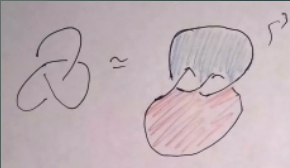
\includegraphics[width=0.8\linewidth]{seifert}
    \caption{Seifert surface of the trefoil knot.}% \label{fig:seifert}
\end{figure}

Here are some more properties of Milnor fibers: \begin{enumerate} \item Each
fiber is parallelizable; \item Each fiber has the homotopy type of a cell
complex of dimension $n$.  \end{enumerate}

\chapter{April 9}% \label{cha:april_9}

Paul used GP/Pari to force Zoom to record at a higher resolution.

\section{More Milnor Fibration}% \label{sec:more_milnor_fibration}

Recall the definition of the Milnor fibration from last time. Then recall that
$F$ is parallelizable and has homotopy type of an $n$-dimensional cell complex.
We give some more properties of the fibration: \begin{enumerate} \item One can
    show that $\pi_1(L), \ldots, \pi_{n-2}(L)$ are all trivial.  \item Each
    fiber is diffeomorphic to an open (in the analytic topology) subset of a
    nonsingular complex hypersurface of the form $f = c$, where $c$ is a
    nonzero constant.  \item Suppose that $0$ is an isolated singularity. Then
    $F$ has the homotopy type of a \textit{bouquet of $n$-spheres}.
    \end{enumerate} Proof of these claims can be found in Milnor's book, but
    they are too long for Paul to give them in class.

The key invariant of an isolated singularity is the \textit{Milnor number}.
\begin{defn}[Milnor number] Let $J_f$ be the ideal generated by the partial
    derivatives of $f$. Then the \textit{Milnor number} is simply \[ \mu
    \coloneqq \dim \C[z_0, \ldots, z_n]/J_f. \] \end{defn}

\begin{defn}[Milnor number, second definition] Let $J: \C^{n+1} \to \C^{n+1}$
    be given by the $\pdv{f}{z_i}$. This induces a map on a smapp sphere
    $S_{\ep}^{2n+1} \to S^{2n+1}$. The degree of the map is the induced map on
    $H_{2n+1}(S^{2n+1})$.  \end{defn}

\begin{thm} The Milnor number $\mu$ is the number of spheres in the bouquet
attached to the isolated singularity. In particular, $H_n(F) = \Z^{\mu}$.
\end{thm}

\begin{exm} The Milnor number of $z_0^2 + x_1^3$ is $2$. From the explicit
drawing of the surface, we can see a homotopy down to a graph with the same
homotopy type as $S^1 \wedge S^1$.  \end{exm}

This is an example of something called a \textit{Brieskorn variety}, which is a
variety of the form $x_0^{a_0} + \cdots + x_n^{a_n}$. In this case, we can
simply compute \[ \mu = (a_0 - 1) \cdots (a_n - 1). \] Recall that we can
consider the monodromy of the fibration. Then this gives an automorphism $h$ of
$F$, and we can regard $h_*: H_n(F) \to H_n(F)$ as an element of
$GL_{\mu}(\Z)$.

\begin{thm}[Deligne-Griffiths] $h_*$ is a unipotent matrix. This means here
that $h_*$ is conjugate to an upper triangular matrix with eigenvalues roots of
unity. Moreover, all Jordan blocks of $h_*$ have dimension at most $n+1$.
\end{thm}

\begin{exm} Let $f = \sum_{i=0}^n z_i^{a_i}$. Then we can explicitly compute
    the eigenvalues of the monodromy map. In fact, they are all products of the
    form \[ \omega_0 \cdots \omega_n, \] where $\omega_i$ is a nontrivial
    $a_i$-th root of unity. For example, in the case $f = z_0^2 + z_1^3$, the
    two eigenvalues are the primitive sixth roots of unity.  \end{exm}

We will now sketch a proof of the formula. First, we can extend the fibration
to all of $\C^{n+1} \setminus V(f)$. We can show that the fiber above $y \in
S^1$ is $F \times \R$. We can now compute the monodromy of this fibration,
which is simply \[ z \mapsto \qty(e^{it/a_0} z_0, \ldots, e^{it/a_n} a_n). \]
Then the monodromy is simply $h_{2\pi}$. By a result of Pham, we see that the
fiber above $1$ deformation retracts onto the \textit{iterated join} of the
$\Omega_{a_i}$. For example, the join of $\Omega_p * \Omega_q$ is simply the
complete bipartite graph $K_{p,q}$.

\begin{exm} If we label some vertices on the Seifert surface we drew last time,
then we can see the graph.  \end{exm}

We can now compute the reduced homology of $F$, and we see that the top
homology is simply \[ \widetilde{H}_n(F) \cong \bigotimes
\widetilde{H}_0(\Omega_{q_i}). \] 

\begin{rmk} Results extend to \textit{weighted homogeneous polynomials} $f$.
    Here, $f(x_1, \ldots, x_m)$ is weighted homogeneous of tope $a_1, \ldots,
    a_m$ if it is a linear combination of monomials $z_1^{i_1} \cdots
    z_m^{i_m}$ where \[ \frac{i_1}{a_1} + \cdots + \frac{i_m}{a_m}. \]
\end{rmk}

\chapter{April 14}% \label{cha:april_14}

Paul calculated $e$ and $\pi$ in GP/Pari.

\section{Globally Symmetric Spaces}% \label{sec:Globally_symmetric_spaces}

\begin{exm} Let $\mc{H}$ be the upper half plane and $\Gamma = SL_2(\Z)$ (or
    some finite-index subgroup), and then we can consider the space $\Gamma
    \backslash \mc{H}$. This is a locally symmetric space, which is simply a
    punctured Riemann surface. There are two obvious compactifications:
\begin{enumerate} \item Fill in the missing points; \item Fill in the missing
points with a bounding circle.  \end{enumerate} Why is this a locally symmetric
space? It is a quotient of a global symmetric space. Here, if $G = SL_2(\R)$
and $K = SO(2)$, then $\mc{H} = G/K$.  \end{exm}

\begin{defn} Let $M$ be a Riemannian manifold with an involution $s_p$ for each
    $p \in M$ that fixes $p$ but reverses every geodesic through $p$. Then we
    call $M$ a \textit{symmetric space}. Note that any such $M$ is complete
    because we can extend geodesics by flipping. Also note that $M$ has a
    transitive isometry group.  \end{defn}

\begin{exm}[Basic Examples] \begin{enumerate} \item $\R^n$ is always a
    symmetric space. Here the geodesics are straight lines and the involutions
    are reflections.  \item Any sphere is a symmetric space.  \item Any
    hyperbolic space $H_n$ is a symmetric space.  \end{enumerate} \end{exm}

\subsection{Classification}% \label{sub:classification}

These spaces were classified by Elie Cartan, which was one of the first major
results in the classification of Lie groups and Lie algebras. Here, $M$ is a
product of three types of symmetric spaces: \begin{itemize} \item Euclidean
    type ($\R^n$); \item Compact type; \item Noncompact type; \end{itemize}
    These are characterized by conditions on their sectional curvature
    (identically zero, nonnegative, nonpositive).

Next, any symmetric space can be factored into irreducible symmetric spaces.
Therefore, we simply need to classify the irreducible symmetric spaces. These
were classified using algebra, and are all $G/K$, where $G$ is a connected Lie
group and $K$ is a maximal compact subgroup.

First, we classify all possible Lie algebras, then see which Lie groups have a
given Lie algebra. Finally, using the theory of root systems and weights, we
obtain $8$ classical families ($A,B,C,D$) of symmetric spaces and $12$
exceptional examples ($E,F,G$). Each one comes in a compact version and a
noncompact version. In fact, there is a duality between the compact spaces and
noncompact spaces.

\subsection{Basic Examples}% \label{sub:basic_examples}

\begin{enumerate} \item Let $G = SL_n(\R)$ and $K = SO(n)$. Then $M = G/K$ and
    has dimension $\frac{(n+2)(n-1)}{2}$. The symmetry comes from the
    involution $X \mapsto (X^{-1})^T$.  \item Let $G = Sp_{2n}(\R)$. Then $K =
    U(n)$ and $M = G/K$ has dimension $n(n+1)$ and is called the Siegel upper
    half-space. This space arises in the study of moduli spaces of abelian
    varieties. In fact, this is a Hermitian symmetric space, which means $M$ is
    a complex manifold.  \item Let $G = SL_2(\C)$ and $K = SU(2)$. Then $G/K =
    H_3$, which is hyperbolic $3$-space.  \item Now consider $G = SL_2(\R)
    \times SL_2(\R)$. Then $K = SO(2) \times SO(2)$ and $H/K = \mc{H} \times
    \mc{H}$. This example and the previous one arise when studying algebraic
    groups over number fields. The upper half-plane corresponds to $\Q$, $H_3$
    corresponds to imaginary quadratic fields, and $\mc{H} \times \mc{H}$
    corresponds to the real quadratic fields. Quotients of $H_3$ give Bianchi
    manifolds, quotients of $\mc{H} \times \mc{H}$ give Hilbert modular
    surfaces, and quotients of $\mc{H}$ give modular curves.  \end{enumerate}

\section{Locally Symmetric Space}% \label{sec:locally_symmetric_space}

Here, we only require involutions that reflect geodesics in neighborhoods of
points. However, every locally symmetric space arises as the quotient of a
global symmetric space by a discrete subgroup of $G$.

\begin{exm} We can consider $G = SL_2(\R)$ and $\Gamma = SL_2(\Z)$.
    Alternatively, we can consider $G = SL_2(\C)$ and $\Gamma = SL_2(K)$ where
    $K$ is an imaginary quadratic field. If $G = SL_2(\R) \times SL_2(\R)$,
    then we can take $\Gamma = SL_2(K)$, where $K$ is a real quadratic field.
    Here, $\Gamma$ acts by $\gamma \cdot g = \gamma g$ on the first factor and
    by $\gamma \cdot g = \overline{\gamma} g$ on the second factor.  \end{exm}

We can understand the geometry of these space by interpreting them as
configuration spaces. We will focus on the case where $G = SL_n(\R)$. Our goal
is to understand compactifications of the locally symmetric spaces
geometrically. Here, points in $\Gamma \backslash X$ correspond to lattices in
$\R^n$ modulo equivalence relations and with some decorations.

\chapter{April 16}% \label{cha:april_16}

Paul computed some values of the Riemann Zeta function.

\section{Compactifications of the Space of Lattices}%
\label{sec:compactifications_of_the_space_of_lattices}

Let $G = SL_n(\R), K = SO(n), \Gamma = SL_n(\Z)$. Then consider the global
symmetric space $X = G/K$. note that any coset $gK$ is a basis of $g$ obtained
by rotation. Therefore $G/K$ corresponds to the set of volume $1$ ordered bases
of $\R^n$ up to rotation. 

Next, consider the locally symmetric space $\Gamma \backslash X$. Here, $\Gamma
g$ gives the lattice generated by the rows of $g$, and thus $\Gamma \backslash
X$ can be identified by the space of lattices in $\R^n$ up to rotation and
scaling.

\begin{rmk} Double coset spaces like $\Gamma \backslash G / K$ are ubiquitous
in geometry. Any double coset space really corresponds to the set of $G$-orbits
on pairs.  \end{rmk}

\begin{proof} Let $X_1 = G/H_1$ and $X_2 = G/H_2$ for two subgroups $H_1,H_2$
    of $G$. Then consider the diagonal action of $G$ by $G: X_1 \times X_2$
    diagonally. Then we can show that $G$-orbits are in bijection with $H_1
    \backslash G / H_2$.  \end{proof}

\begin{exm} Let $G = SL_n(\C)$ and $B$ be the maximal Borel subgroup. Then
    $G/B$ is the flag variety, and $B \backslash G / B$ encodes the relative
    positions of two flags in $\C^n$. The Bruhat decomposition shows that this
    is actually a finite set, indexed by the Weyl group $W$.  \end{exm}

\begin{exm} Consider $G = SL_n(\R)$ and $K = SO(n)$. Then we can encode $X =
    G/K$ as the set of volume $1$ ellipsoids in $\R^n$ and the points give
    metrics on $\R^n$. Then the space $K \backslash G / K$, which parameterizes
    ellipsoids of volume $1$ up to rotation. By a result of Euler, this is
    paramaterized by positive real numbers whose product is $1$.  \end{exm}

Therefore, we can consider $\Gamma \backslash G / K$ as the set of $G$ orbits
in $G/\Gamma \times G/K = \{ \text{lattices} \} \times \{ \text{metrics} \}$.
We can consider the space of lattices in the presence of a fixed metric or the
space of metrics in the presence of a fixed lattice.

\begin{rmks} The space $\Gamma \backslash X$ is very close to being a manifold.
    It has singularities, but they are very mild (in fact just quotient
    singularities), so the space is an orbifold. The singularities come from
    lattices with nongeneric symmetry (with symmetry that is more than just $x
    \mapsto -x$).

    \begin{enumerate} \item We can give up and call this space an orbifold,
        stack, or some other new term, or we can incorporate decorations with
        the lattices. We will take the second approach later. This corresponds
        to replacing $SL_n(\Z)$ with a finite index subgroup.  \item This space
        is not compact. If we scale the $x$-axis up and the $y$-axis down, this
        sequence of lattices clearly does not converge. In fact, a theorem of
        Mahler says that a sequence of lattices diverges to infinity if and
        only if the length of the minimal nonzero vector converges to $0$.
\end{enumerate} \end{rmks}

\subsection{Topology and Geometry for Small $n$}%
\label{sub:topology_and_geometry_for_small_n_}

Let $n = 2$. Then this gives lattices in $\R^2$ modulo rotation and scaling. We
are looking for a fundamental domain for $\Gamma$ acting on $X$ together with
an identification on its boundary. This is known as explicit reduction
theory.\footnote{This supposedly has applications in the ``real world,''
whatever that is. There was a remark about how GPS is useless now because we're
all sitting at home.}

First, we will find a shortest nonzero vector $v \in L$. If we rotate and scale
$v$ onto $e_1$, we can choose the minimal length vector $w$ from the row
immediately above the $x$-axis. Then $\abs{w} \geq 1$ and lies in the strip
between $-\frac{1}{2}$ and $\frac{1}{2}$. This gives the famous picture of the
fundamental domain in the upper half plane. The two vertical lines are clearly
identified, and then the arc the arc is folded in half. Therefore, the space
$\Gamma \backslash X$ is topologically equivalently to a disc.


\chapter{April 21}% \label{cha:april_21}

Paul computed some values of $L$-functions of number fields in GP/Pari. He then
mentioned the class number formula.

Last time, we discussed the space of lattices modulo rotation and scaling. In
addition, we computed the fundamental domain of the action of $SL_2(\Z)$ on the
upper half-plane.

\section{Geometry for $n=3$}% \label{sec:geometry_for_n_3_}


We now consider the space of lattices in $\R^3$. We can rescale to make the
shortest nonzero vector $(1,0,0)$. Then we can rotate the next shortest vector
to lie in the $xy$-plane, and we can assume that $v_2$ is in the right half of
the fundamental domain of $SL_2$. Finally, we choose a $v_3$ lying above the
plane. To do this, consider the quotient of $\R^3$ by the plane, and we can
choose $v_3$ in the inverse image of the shortest nonzero vector in the
quotient lattice.

\begin{rmk} The image of a lattice in a quotient space is not necessarily a
lattice.  \end{rmk}

Next, we consider where we can arrange $v_3$ to be. We can move along the
lattice and move $v_3$ to lie over a polygon determined by $v_1,v_2$. In
addition, $v_3$ cannot lie inside the unit hemisphere. Therefore, our
configuration has dimension $5$ and should have a deformation retract onto a
compact space of dimensnio $3$.

First, let's ignore the noncompact dimensions and focus on the compact part. To
see this object, we move $v_2$ to the top of the semicircle and look at the
possible polygons. Here, the polygon is the set of points whose distance to the
origin is smaller than the distance to any other lattice points. This is called
the Dirichlet-Voronoi domain.\footnote{Paul discussed real-world applications
of these things.} Then this three dimensional space is very complicated, and it
is easier to describe a finite version. This is simply a cube with four of the
vertices truncated. Note the center of the triangular face is the $A_1 \times
A_1 \times A_1$ lattice while the center of a hexagonal face is the $A_2 \times
A_1$ lattice.

\begin{figure}[H] \centering 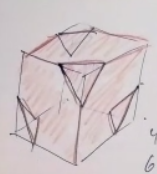
\includegraphics[scale=0.5]{voronoi.png}
    \caption{Soul\'e's cube. This was used to compute the cohomology of
    $SL_3(\Z)$.}% \label{fig:name} \end{figure}

\begin{exer} Find the three remaining special lattices (names can be found in a
crystollagraphy book).  \end{exer}

We will not consider the higher-dimensional analogues. The quotients are
well-understood up to $n=7$, but the case $n=8$ is unknown. In $n=8$, we have
the $E_8$ lattice, which makes the geometry of the polytope extremely
complicated.\footnote{Paul said that $E_8$ is a legitimate excuse for not doing
anything.} We have no idea how many faces there are, but we do have a few crude
estimates. In addition, our algorithm for finding a nice basis of our lattices
fails in dimension greater than $3$. It barely works for $n=4$, but fails for
$n=5$.

\begin{exm} Consider the lattice $L \subset \R^5$ with basis $e_1, e_2, e_3,
    e_4, \frac{1}{2} (e_1 + \cdots + e_5)$. Note that $\Z^5$ is a strict subset
    of $L$. However, if we run our algorithm, we only obtain the $\Z^5$
    lattice, which is not $L$.  \end{exm}

\begin{rmk} Even worse, in high dimensions, there exist lattices such that
\textbf{no} basis contains a minimal vector (Conway-Sloane).  \end{rmk}

\section{Singularities of the space of lattices}%
\label{sec:singularities_in_gamma_backslash_x_}

We can eliminate these singularities by introducing extra data. We will call
these ``marked lattices'' and our extra data will kill these automorphisms.

\begin{defn} A \textit{marking} on a lattice is a surjective map $m:L \to S$
such that there exists a finite index sublattice $L'$ such that $m$ is fixed by
translation by $L'$.  \end{defn}

\begin{exm} We can mark $L = \Z^n$ using $S = (\Z/p\Z)^n$ by reduction mod $p$.
Here, $L' = p\Z^n$.  \end{exm}

\begin{rmk} We can think of markings as coming from coloring data on our
lattices.  \end{rmk}

We can consider ``$\Gamma(p)$ markings.'' Then the space of marked lattices is
\[ \bigsqcup_{i \text{ finite}} \Gamma_i \backslash X, \] where $\Gamma_i$ is a
finite-index subgroup.

\begin{thm} For $p \geq 3$, all $\Gamma(p)$-marked lattices have the same
automorphisms. Therefore, the moduli space of marked lattices is smooth. The
analogous procedure for abelian varieties is taking a principal polarization.
\end{thm}

\chapter{April 23}% \label{cha:april_23}

\section{Compactifications of Locally Symmetric Spaces}%
\label{sec:compactifications_of_locally_symmetric_spaces}

\begin{exm} Consider $\R^n$. How do we compactify it? How do we add limit
    points for rays that go off to infinity? If the lines are parallel, do we
    want them to have the same limit point? This is one of the reasonable
    ideas, and we obtain a $S^{n-1}$ at infinity.

    If we forget about rays and just consider lines, we obtain $\P^n(\R)$, with
a $\P^{n-1}(\R)$ at infinity. In both these examples, we see that points at
infinity can be recorded via equivalence relations on geodesics.  \end{exm}

\begin{exm} Let $\Gamma = \Z/6\Z$ act on $\R^2$ by rotation. Then note that any
    cone with angle $\pi/3$ is a fundamental domain. How do we compactify this?
    \begin{description} \item[Method 1:] We use what we did for $\R^2$. We can
        extend the action to the compactification of $\R^2$ (say the $S^1$) at
        infinity, and we obtain an honest cone.  \item[Method 2:] We now have
        $6$ distinguished rays. We can attempt to use the $1$-parameter family
        of parallel rays for each of these. Now we glue these $6$ lines onto
        $\R^2$. We will dictate that the two rays bounding one fundamental
        domain give lines that intersect at a single point. All rays between
        the two distinguished rays will converge to that single point. In some
        sense, this is dual to what we did before and we have a hexagon at
        infinity.  \end{description}

    Why would we consider the second method?  \begin{enumerate} \item We gain
        information that we lost in the first method.  \item This is what
        happens when we consider toric varieties.  \item When we consider
        $\Gamma \backslash X$, we need something more like this method.
\end{enumerate} \end{exm}

Now we will consider the space of lattices up to rotation and scaling. Here,
our points have a geometric interpretation, so we can try to leverage this. We
have two tools to work with: \begin{enumerate} \item Geodesics in $\Gamma
    \backslash X$. We can think of adding limit points for families of
    geodesics.  \item In configuration spaces and moduli problems, we want the
    points at infinity to have a geometric meaning.\footnote{\textbf{Note
    Taker:} See for example the space $\overline{M}_{g,n}$.} For us, this means
    that lattices should degenerate to something more general. There are other
    contexts: \begin{enumerate} \item Consider the moduli space of genus $g$
        curves $M_g$. When we go to infinity, we pass to stable nodal curves
        with several components.  \item Consider the moduli space of abelian
        varieties. These degenerate to various geometric objects.
\end{enumerate} \end{enumerate}

Now if we consider lattices in $\R^2$, consider the family of lattices $L(t) =
\ev{2^{-t} v_1, 2^t v_2}$, this should converge to the $x$-axis at infinity and
the $y$-axis at $-\infty$. The moral of the story is that lattices degenerate
to subspaces. This may not seem too complicated for $n=2$, but it is very
complex when $n=3$.

\begin{rmk} This approach does use geodesics! We are moving around in the upper
half-plane.  \end{rmk}

Now we consider the space of lattices in $\R^3$. Recall this is isomorphic to a
quotient of the Soul\'e cube times $(\R_{\geq 0})^2$. If we start with the
standard basis vectors, we can consider the family \[ L(t) = \gen{2^{-t} e_1,
2^{-t}e_2, 2^{2t}e_3}.\] As $t \to \infty$, we simply obtain the $xy$-plane.

For another example, consider \[ L(t) = \ev{2^{-2t}e_1, 2^t e_2, 2^t e_3} .\]
In the limit at infinity, we simply obtain the $x$-axis. We can also see ``in
between'' phenomena. Consider the family \[ L(t) = \ev{2^{-3t}e_1, 2^{-2t} e_2,
2^{5t} e_3}. \] We can see that the $x$-direction collapses faster than the
$y$-direction, so if we rescale by $2^{2t}$, we see that the limit is a flag $0
\subset (y=z=0) \subset (z=0)$. 

\begin{rmk} We have seen all possible degeneration types. Now we can attempt to
    look for more refined degeneration data. We observe that the image of the
    diagonal matrices in $SL_3(\R) / SO(3)$ is a maximal flat geodesic
    submanifolds. Therefore, the points at infinity should be parameterized by
    flags with some extra data.  \end{rmk}

If we return to the first example $L(t) = \gen{2^{-t}e_1, 2^{-t}e_2,
2^{2t}e_3}$. Recall that we obtain the plane as the limit. However, for $t \gg
1$, the images of $e_1, e_2$ give a lattice in the plane. This gives a point in
our space for $n=2$! If we change $e_1,e_2$ to different $v_1,v_2$ (say the
basis for the $A_2$ lattice), then we obtain a different lattice in our
intermediate stage.

\chapter{April 28}% \label{cha:april_28}

Last time we discussed limits of lattices in $\R^n$. We were able to obtain
flags by degenerating lattices. Unfortunately, not every flag can arise as the
degeneration of a lattice family.

\begin{exm} Consider $n=2$ with $X = \mc{H}$. Then suppose $\Gamma = SL_2(\Z)$.
    Suppose we head down to $\alpha \in \R$ along a geodesic. If $\alpha$ is
    rational, then we go off to infinity. However, if $\alpha$ is irrational,
    the picture is much more subtle.  \begin{itemize} \item If $\alpha$ is
        contained in a real quadratic field, then the path approaches a
        periodic geodesic.  \item Otherwise, the path wanders around the
        quotient and does not escape to infinity. The behavior here is
        completely unknown.  \end{itemize} \end{exm}

In terms of flags, only certain flags will arise as limit points, and in fact,
we want \textit{rational flags}. These are flags whose subspaces are generated
by lattice points. What about limiting shapes of lattices?

When $n=3$, we have three types of limiting flags: a plane, a line, and a line
inside a plane. When we have a plane, we have a shape inside the limiting
plane. In the case of a line, we expect a shape inside the quotient of $\R^3$
by the line. Finally, in the case of a full flag, we expect no shape data. More
generally, for a flag \[ 0 = F^1 \subsetneq F^2 \subsetneq \cdots \subsetneq
F^k = \R^n, \] we can look at pairwise successive quotients and find lattice
shapes there. Putting it all together, we obtain the reductive Borel-Serre
compactification. Strata are induced by rational flags in $\R^n$ including the
empty flag.

For example, we can add three different types of strata when $n=3$. We can
index them by partitions of $3$ where the order of the parts matters.
\begin{table}[H] \centering \caption{Partitions and Strata} \label{tab:label}
    \begin{tabular}{ccc} \toprule Flag & Partition & Strata \\ \midrule
        $\emptyset$ & $3$ & $5$-dimensional strata \\ $\R^2$ & $2+1$ &
        $2$-dimensional strata at infinity \\ $\R^1$ & $1+2$ & $2$-dimensional
        strata at infinity \\ $\R^1 \subset \R^2$ & $1+1+1$ & $0$-dimensional
        strata at infinity \\ \bottomrule \end{tabular} \end{table} In fact,
        the strata at infinity are lower-rank locally symmetric spaces that are
        being compactified themselves in this process. The space for $n=3$
        looks something like this: \begin{figure}[H] \centering
            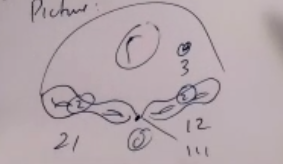
\includegraphics[width=0.8\linewidth]{space.png}
            \caption{Simplified picture of strata for $n=3$}%
        \label{fig:Simplifi} \end{figure} This space is singular. We have
        attached two-dimensional strata to a five-dimensional space. We can
        compte links by realizing the space as a quotient of a manifold with
        corners. The bigger space is called the Borel-Serre
        compactification.\footnote{Apparently this was part of one of only two
        papers jointly written by Borel and Serre.} There will be a
        five-dimensional stratum and two four-dimensional strata that meet in a
        three-dimensional corner. In fact, the four-dimensional strata are
        fiber bundles over the locally symmetric spaces for $n=2$.

Consider the case when $n=2$. Suppose $\gamma_1, \gamma_2$ are parallel
geodesics that go off to infinity. Should they go to different limiting points
or the same point? Recall our discussion about compactifying $\R^n$. There are
two answers here: \begin{enumerate} \item We can send them to the same point
    because of the metric on the upper half plane. This is because the two
    geodesics get arbitrarily close together.  \item The geodesics hit
    different points on various parallel horocycles.\footnote{Apparently
    electrical engineers use geodesics and horocycles on the hyperbolic plane
as graph paper on a disc.} Thus sending them to different points also makes
sense.  \end{enumerate} To add this data in our lattice/flag description, we
add a \textit{real} transverse flag to the data. The transverse flag
corresponds to adding an $S^1$ at infinity. This $S^1$ is really the matrices
of the form \[ \begin{pmatrix} 1 & x \\ 0 & 1 \end{pmatrix} \in SL_2(\R). \] In
the quotient, this circle is collapsed down to a point.

When $n=3$, we add flags to the strata corresponding to the compositions
$21,12,111$. In the Lie groups picture, the three strata correspond to
parabolic subgroups. Then the fiber above each point in the two dimensional
strata is a torus. Then the three-dimensional stratum is the image of the
matrices of the form \[ \begin{pmatrix} 1 & * & * \\ 0 & 1 & * \\ 0 & 0 & 1
\end{pmatrix} \] and is called a nilmanifold of the Heisenberg manifold.

\begin{exer} Compute the links of points in the strata using the presentation
as a space with thin singularities.  \end{exer}

\begin{rmk} It is an open question to generalize these constructions to the
    nonarchimedean setting. Here, we want to replace real Lie groups with
    reductive groups over $\Q_p$ and $K$ with the same group over $\Z_p$. For
    example, we replace $SL_n(\R)$ with $SL_n(\Q_p)$ and $K = SO(n)$ with
    $K=SL_n(\Z_p)$. The analogue of $X$ in this setting is called a
    \textit{building}. Compactifications of $X$ in this setting have been
    studied, but locally summetric spaces have not been studied.  \end{rmk}

\end{document}
